\chapter{\textbf{Scenario Implementation and Results}}
% Introduction
This chapter presents results of two trajectories using the proposed navigation filter and its underlying components discussed in previous chapters. Each trajectory is subject to varying degrees of signal interference across multiple Monte-Carlo simulations. First, an overview of the Monte-Carlo analyses that will be presented for each trajectory is provided. Next, a discussion of the first trajectory and configuration file used for the simulations is presented. Following a description of trajectory one, Monte-Carlo analyses highlight the strong and weak points of the proposed navigation filter. Once the analyses of the first trajectory conclude, a description of trajectory two is presented, followed by a similar Monte-Carlo statistical analysis. Each Monte-Carlo case is composed of 100-run simulations for each trajectory subject to seven cases of signal degradation. To show the improved performance of the proposed navigation filter, a constant-velocity, kinematic model VDFLL~\cite{grierPositionNavigationTiming} is shown as a comparison. This standard VDFLL processes the same trajectories at the same cases of signal degradation.

\section{\textbf{Monte-Carlo Analyses}}
Originally named after a famous casino in Monaco, the Monte-Carlo analysis is a model to predict the probability of an outcome given the presence of random variables~\cite{mariettaMonteCarloError2013}. For the deeply-coupled FVDM, a number of random variables exists. For one, the true states of the aircraft are disturbed by wind, causing the aircraft to veer from the desired target line, that is, between simulations, the simulated aircraft will not fly the same flight path every time, regardless of having the same set of waypoints. For the purpose of this work, these wind disturbances are modeled with the same magnitude {--} interference and trajectory notwithstanding. Within the VT algorithms, the correlator simulator features noise that occurs at every measurement step, meaning no correlators (Equation~\ref{eq:correlators}) will be the same between simulations for the same time step. For the correlator simulation tool presented in this thesis, the random noise placed onto the correlators is a function of the interference level. As demonstrated by Equation~\ref{eq:CN0}, higher variance noise when compared to the amplitude of the cross-correlated local and received signal leads to an overall lower \(C/N_0\) ratio, which is demonstrated by the results later on in this chapter.

For each of the trajectories presented in this chapter, the 100-run Monte-Carlo simulations will evaluate the two different navigation filters for their probability to track the GPS signal given \(C/N_0\) degradation. Furthermore, Monte-Carlo analysis on code phase and carrier frequency error over a range of \(C/N_0\) values is presented. For the pose and attitude estimation results, the Monte-Carlo simulation will provide an average Latitude, Longitude and Altitude estimate compared to the true state of the receiver, along with velocity magnitudes (speed) for the same comparison. As will be discussed later, one of the benefits in using the proposed navigation solution is the ability to estimate angular rates and Euler attitude of the aircraft during simulation. The Monte-Carlo analysis will present the average error in comparison with the true angular rates and Euler attitude as well, but only for the deeply-coupled FVDM, as the standard VDFLL implementation does not have this capability. Lastly, the Monte-Carlo analysis of the 100-run simulations will compare the clock bias and clock drift estimates from both filters compared to the true clock bias and clock drift of the embedded OCXO on board.


\section{\textbf{First Trajectory}}
For the first trajectory, the aircraft is simulated for a straight flight path while maintaining a constant altitude of 500 meters above sea level (Figure~\ref{fig:trajectory1}).

\begin{figure}[!ht]
    \centering
    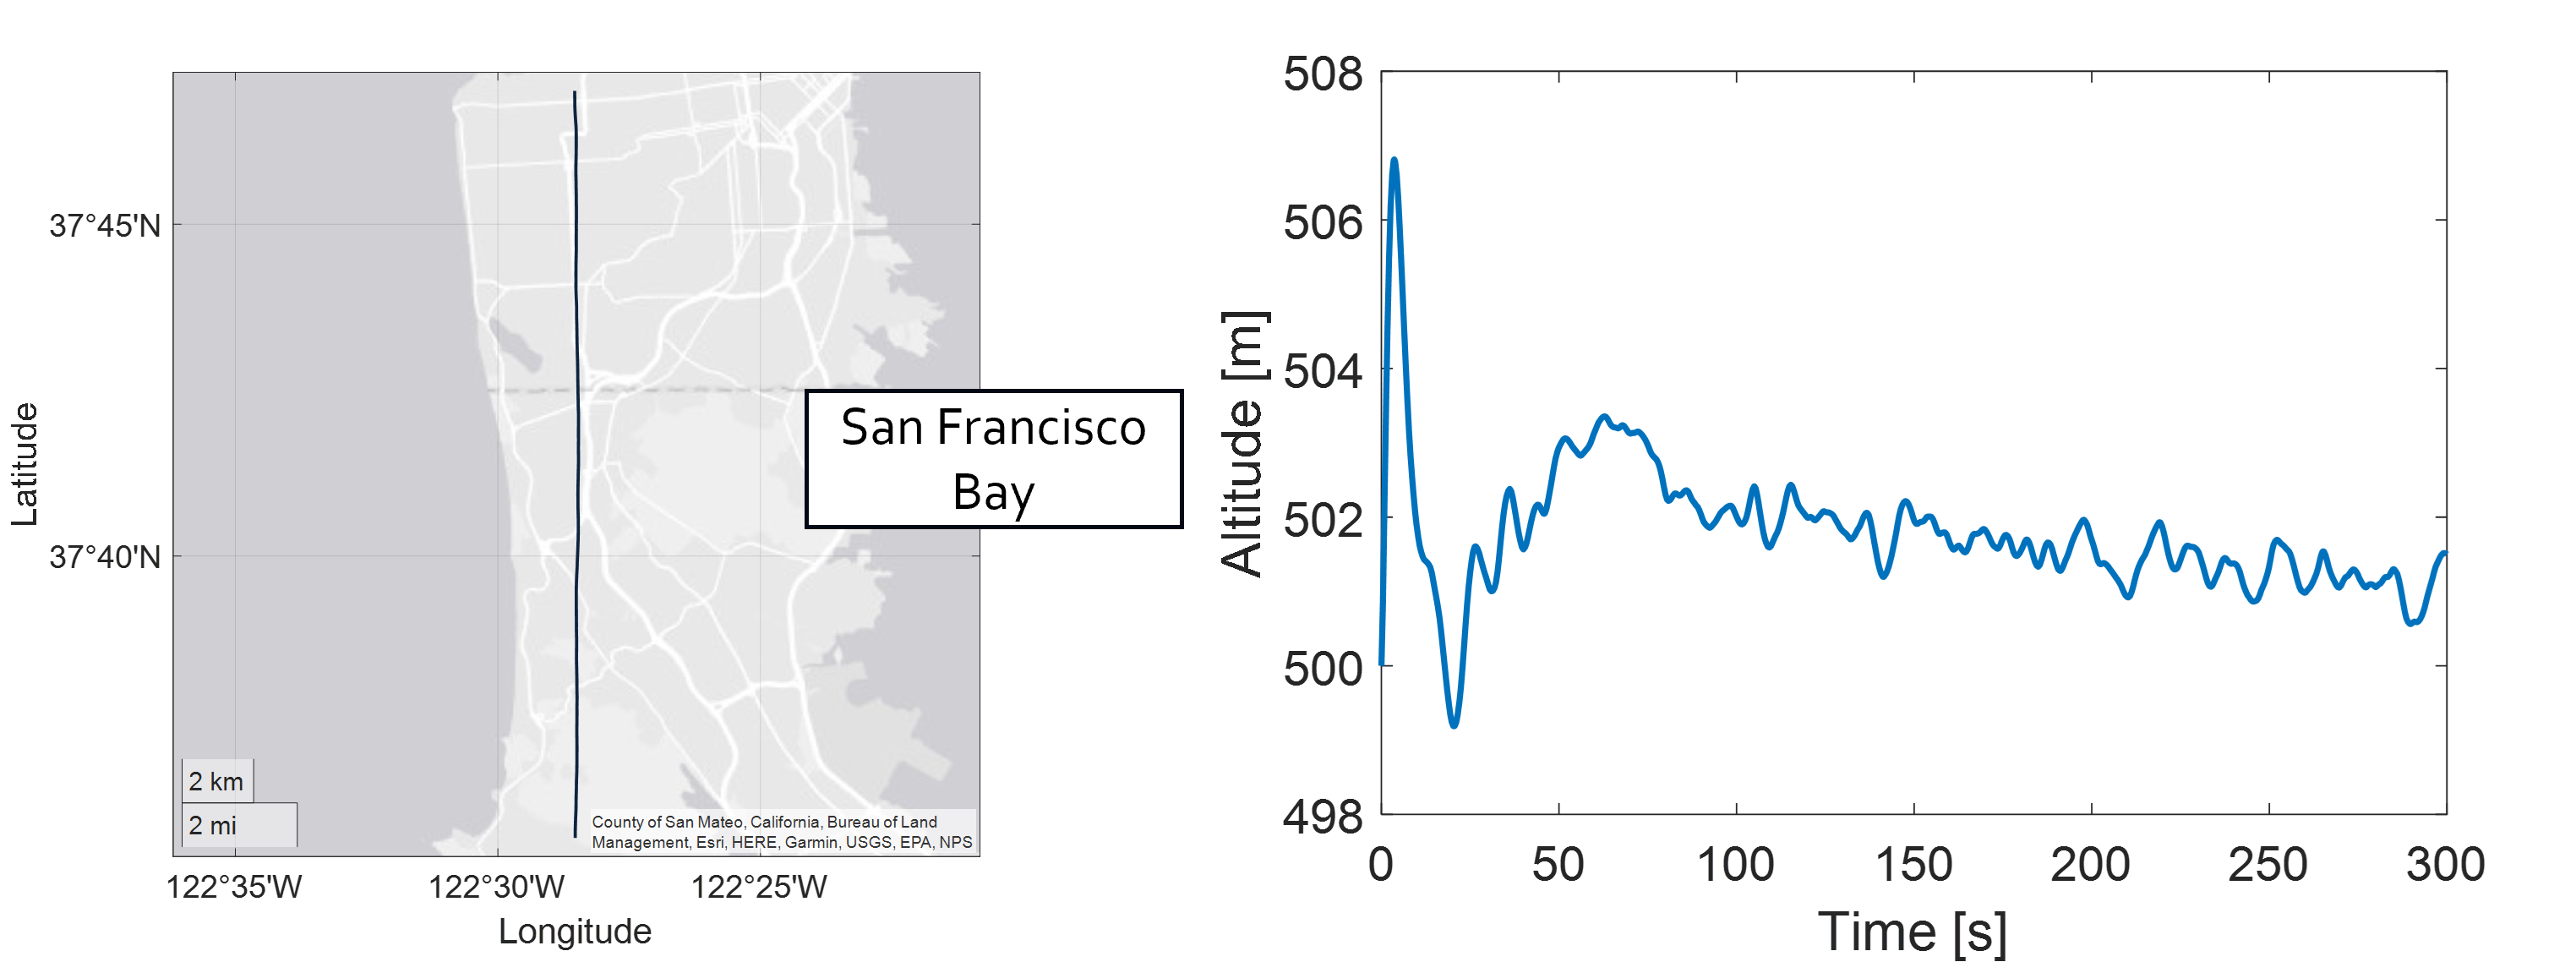
\includegraphics[width=0.9\linewidth]{Figures/Results/trajectory1.png}
    \caption{(Left) Top-view of simulated flight path for trajectory one. (Right) Altitude of flight path for trajectory one.}\label{fig:trajectory1}
\end{figure}

It is assumed that the initial position of the receiver is known when the simulation begins, avoiding the need to perform scalar tracking loops on the received signal data as discussed previously. For the first trajectory, the receiver aboard the aircraft is subject to seven different cases of interference that degrade the signals from the nine tracked channels (Table~\ref{tbl:interferenceCases}). The receiver is subject to these degraded power levels for the entirety of the 60 second simulations.

\begin{table}[!ht]
    \caption{Signal power for each case applied to each trajectory.}\label{tbl:interferenceCases}
    \centering
    \begin{tabular}{cc}
        \toprule
        Case & \(C/N_0\) [dB-Hz] \\
        \midrule
        1    & 45                \\
        2    & 35                \\
        3    & 25                \\
        4    & 22                \\
        5    & 20                \\
        6    & 18                \\
        7    & 16                \\
        8    & 15                \\
        9    & 10                \\
        10    & 5                \\
        11    & 2                \\
        \bottomrule
    \end{tabular}
\end{table}

From Table~\ref{tbl:trajectory}, several parameters are configurable to meet the desired simulation of the user.

\begin{table}[!ht]
    \caption{Initial conditions for simulated trajectory from Figure~\ref{fig:trajectory1}.}\label{tbl:trajectory}
    \centering
    \begin{tabular}{lcc}
        \toprule
        \textbf{Condition}       & \textbf{Value}                                      & \textbf{Units}                     \\
        \midrule
        Date                     & June 15, 2022                                       & \textit{DateTime} Object           \\
        Duration                 & 300                                                 & \(s\)                              \\
        Monte-Carlo Runs         & 100                                                 & {--}                               \\
        Frequency                & 200                                                 & Hz                                 \\
        Trajectory               & \textit{StraightFlightPath.mat}                     & See Chapter 5                      \\
        Velocity Disturbance     & \(\left[300, \; 300, \; 0\right]\)                  & \(m/s\)                            \\
        Angular Rate Disturbance & \(\left[10^{-12}, \; 10^{-12}, \; 10^{-12}\right]\) & \(rad/s\)                          \\
        Clock Type               & OCXO                                                & {--}                               \\
        Initial Velocity         & \(\left[75, \; 0, \; 0\right]\)                     & \(m/s\)                            \\
        Initial Angular Rate     & \(\left[0, \; 0, \; 0\right]\)                      & \(rad/s\)                          \\
        Initial Position         & \(\left[0.65617, \; -2.1376, \; 500\right]\)        & \(\left[rad, \; rad, \; m\right]\) \\
        Initial Attitude         & \(\left[0, \; 0, \; 0\right]\)                      & \(rad\)                            \\
        Initial Clock Terms      & \(\left[0, \; 0\right]\)                            & \(\left[m, \; m/s\right]\)         \\
        Channel \(C/N_0\)        & \(45,\,35,\,25,\,22,\,20,\,18,\,16,\,15,\,10,\,5,\,2\)                & dB-Hz                              \\

        \bottomrule
    \end{tabular}
\end{table}
Date is used to pull the specified Rinex file from~\cite{nollCrustalDynamicsData2010}. This Rinex file is then parsed for its ephemeris and used to propagate the GPS satellites during the simulation. Figure~\ref{fig:skyplot} shows the available satellites at the first time step for June 15, 2022 used in this work.

\begin{figure}[!ht]
    \centering
    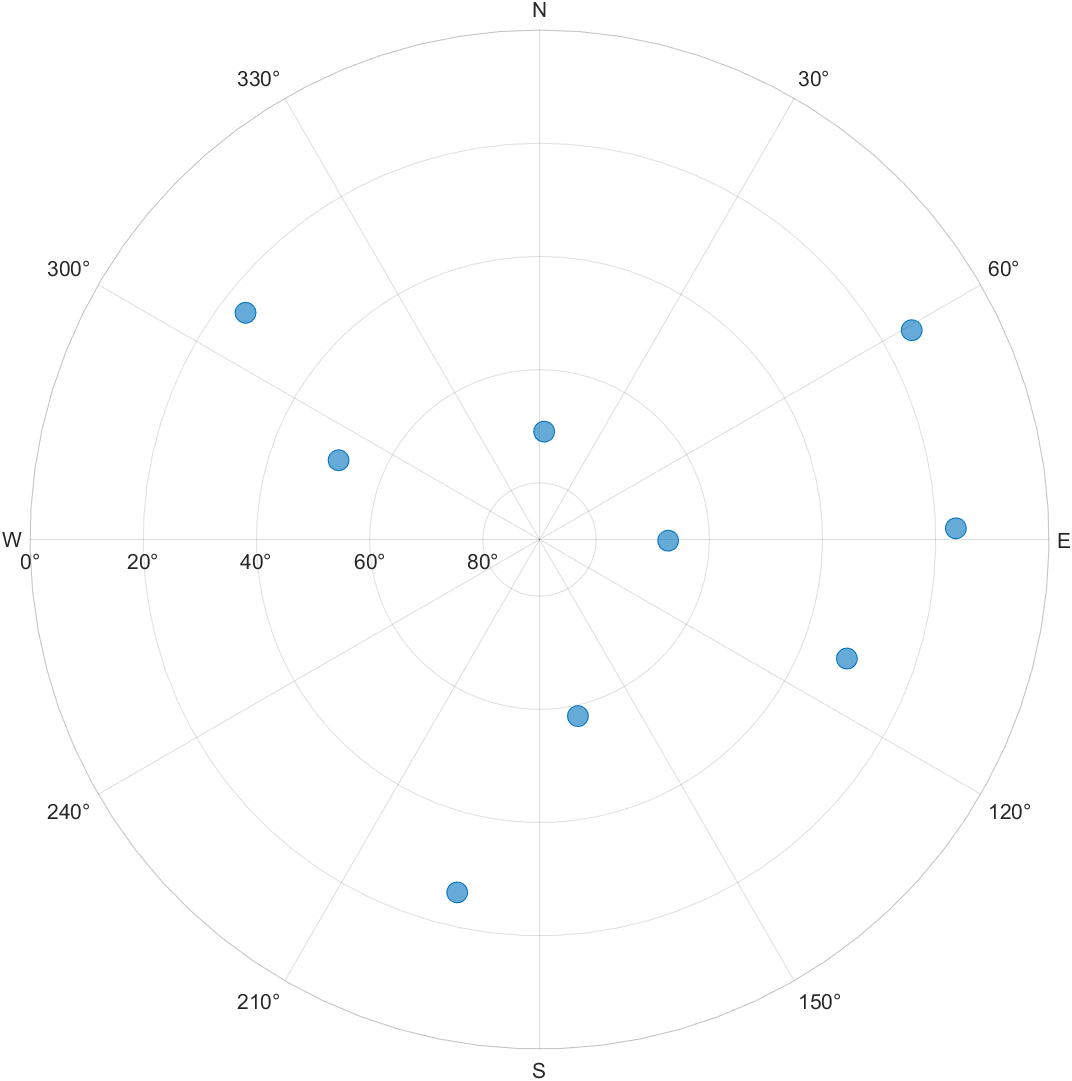
\includegraphics[width=0.8\linewidth]{Figures/Results/skyplot.png}
    \caption{Orange dots signify satellite locations at the start of the simulations given the date of broadcast ephemeris. Black dots signify satellites that are in-view but are discarded due to the 10 degree mask angle used. The green triangle represents the initial receiver position.}\label{fig:skyplot}
\end{figure}
Duration and Monte-Carlo Runs specify the length of each simulation in seconds and the number of simulations for each scenario and/or case. For the work presented in thesis, 100 simulation Monte-Carlo runs are used for analyses. Based on~\cite{khaghaniAssessmentVDMbasedAutonomous2018,khaghaniAutonomousVehicleDynamic2016,mwenegohaModelbasedTightlyCoupled2020} and time to completion for each simulation, 100 is enough to show the general trend for statistical purposes. The trajectory is specified as a -mat file. The creation of the trajectory is detailed in Chapter 5. Trajectory one is a baseline case where it is expected that both the deeply-coupled FVDM and constant-velocity kinematic model both perform well.  As explained in Chapter 5, disturbances are modeled onto the trajectory of the aircraft as the FVDM is not perfect. External conditions such as wind and various atmospheric effects alter the behavior of the Diamond DA-40 slightly. These disturbances are defined as Velocity and Angular Rate in Table~\ref{tbl:trajectory}. Clock Type is the embedded receiver clock modeled during the simulation. More information on the different types of clocks can be found in Chapter 4. For the purposes of this thesis, both trajectories and all cases of signal interference will use the OCXO as the embedded receiver oscillator. The initial states of the aircraft are defined by the given values. Since our trajectory specifies a mostly-north flight path, the north velocity component is specified to be 75 meters per second, while the other components are zero. Also, the pitch of the aircraft is specified as 4 degrees up, this is so the aircraft generates lift at the beginning of the simulations and does not enter a stall upon initialization. Lastly, the initial position of the aircraft is specified as the first waypoint location, for simplicity. The last configurable parameter is the initial channel \(C/N_0\) of the available satellites.


\subsection{\textbf{Monte-Carlo Analyses}}
From the Monte-Carlo results, several parameters can be analyzed for the performance improvements of the proposed navigation filter over the standard VDFLL kinematic model. This section begins with a comparison of the tracking-level results of the two filters subject to different levels of signal degradation.

For the range of signal interference presented in Table~\ref{tbl:interferenceCases}, the Root Mean Square Errors (RMSE) of both the code phase and carrier frequency shows the improved performance by using the deeply-coupled FVDM in GPS-challenged environments (Figure~\ref{fig:codecarrierstraight}). During simulations where the signal was slightly degraded or benign (i.e.\ channel power greater than \(35\) dB-Hz) the standard velocity implementation of the VDFLL actually performs better on average than the proposed navigation filter. This is most likely due to the FVDM becoming over confident during simulation. This is more evident from Tables~\ref{tbl:straight35FVDM} and~\ref{tbl:straight35CV} where the position RMSE, STandard Deviation (STD), and maximum error from the constant velocity kinematic model are marginally better.

\begin{figure}[!ht]
    \begin{subfigure}{.45\textwidth}
        \centering
        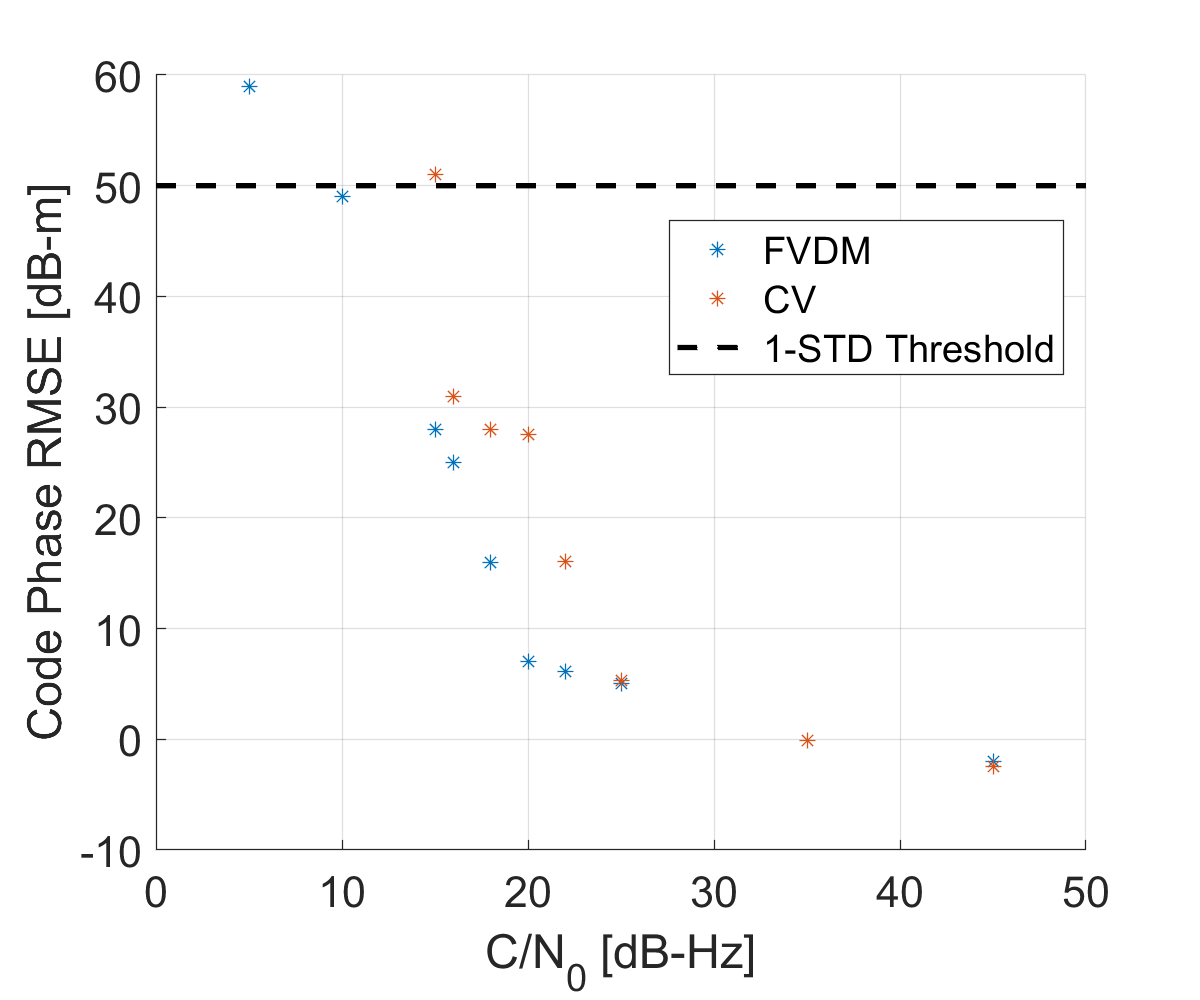
\includegraphics[width=1\linewidth]{Figures/straight/codephaseRMSEstraight.png}
    \end{subfigure}%
    \begin{subfigure}{.45\textwidth}
        \centering
        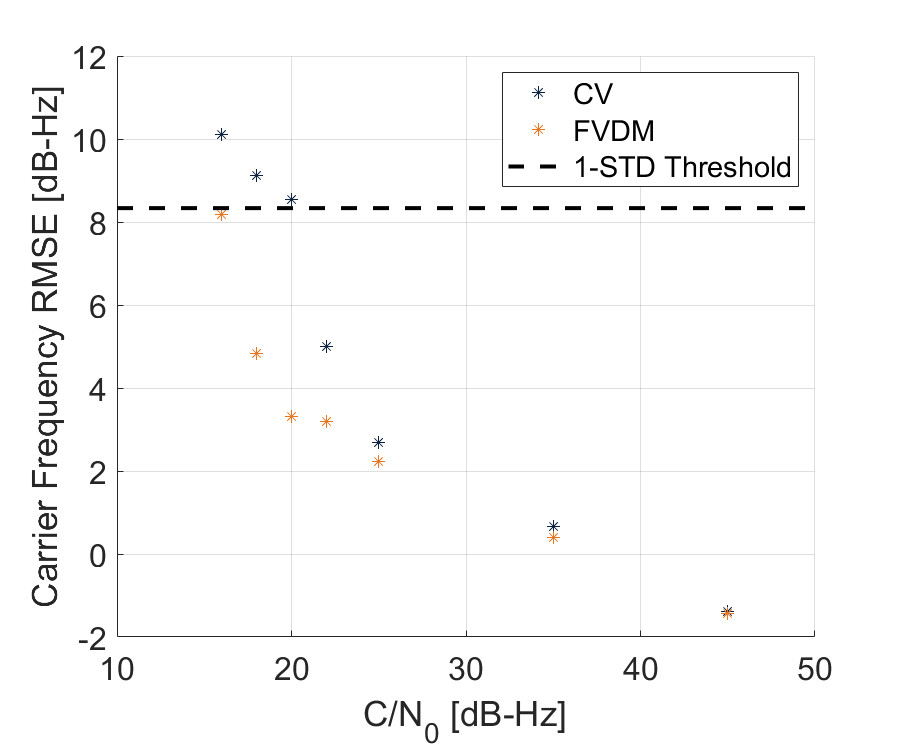
\includegraphics[width=1\linewidth]{Figures/straight/carrFreqRMSEstraight.png}
    \end{subfigure}
    \caption{Code phase and carrier frequency RMSE as a function of signal power, specified in dB-Hz.}\label{fig:codecarrierstraight}
\end{figure}

\begin{table}[!ht]
    \caption{RMSE, STD, and maximum error from 100-run Monte Carlo simulation when the deeply-coupled FVDM is subject to a degraded signal power level of \(35\) dB-Hz.}\label{tbl:straight35FVDM}
    \centering
    \begin{tabular}{ccccc}
        \toprule
                  & Position [m] & Speed [m/s] & Clock Bias [m] & Clock Drift [m/s] \\
        \midrule
        RMSE      & 0.23443      & 0.066059    & 0.013062       & 0.002834          \\
        STD       & 0.11305      & 0.030674    & 0.17509        & 0.0032795         \\
        Max Error & 0.72197      & 0.22588     & 0.05835        & 0.009             \\
        \bottomrule
    \end{tabular}
\end{table}

\begin{table}[!ht]
    \caption{RMSE, STD, and maximum error from 100-run Monte Carlo simulation when the standard VT receiver is subject to a degraded signal power level of \(35\) dB-Hz.}\label{tbl:straight35CV}
    \centering
    \begin{tabular}{ccccc}
        \toprule
                  & Position [m] & Speed [m/s] & Clock Bias [m] & Clock Drift [m/s] \\
        \midrule
        RMSE      & 0.093008     & 0.087402    & 0.013897       & 0.0032735         \\
        STD       & 0.048771     & 0.038728    & 0.015186       & 0.0040279         \\
        Max Error & 0.25751      & 0.26045     & 0.033083       & 0.009487          \\
        \bottomrule
    \end{tabular}
\end{table}

However, when the signal power is less than \(35\) dB-Hz, the deeply-coupled FVDM presents steady performance improvements as the interference grows stronger. For carrier frequency error, the deeply-coupled filter breaks down at roughly \(16\) dB-Hz, where the theoretical \(8.33\) dB-Hz STD from~\cite{lashleyPerformanceAnalysisVector2009} is met. For the standard VDFLL implementation, this criteria is met at roughly \(20\) dB-Hz. The probability that the vector tracking loops are able to maintain channel lock for an entire simulation is shown in Figure~\ref{fig:trackingprobability1}.

\begin{figure}[!ht]
    \centering
    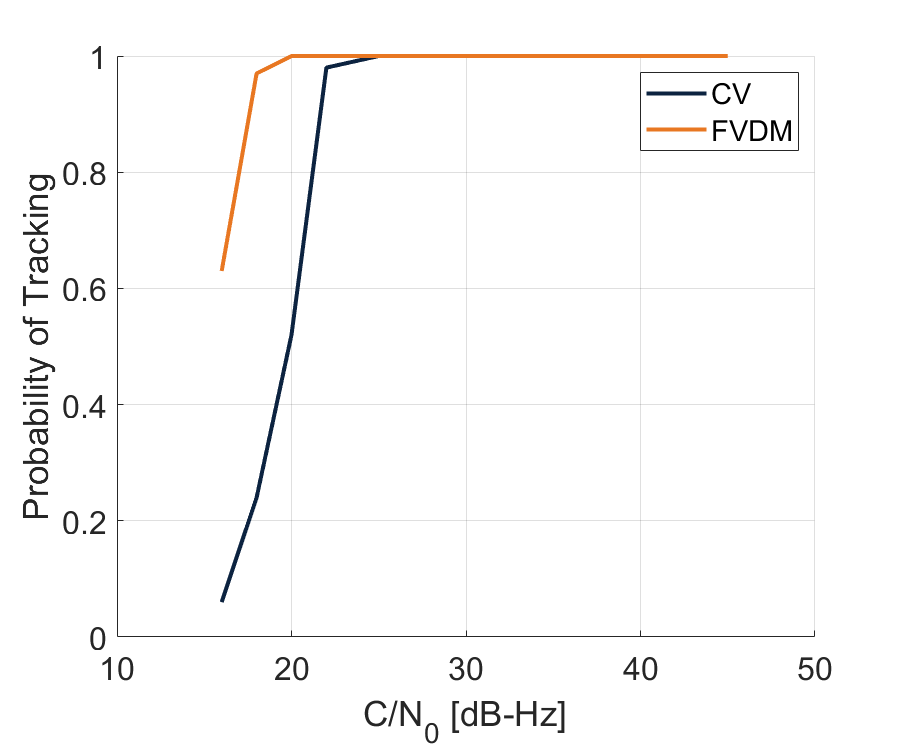
\includegraphics[width=0.5\linewidth]{Figures/straight/trackingprobstraight.png}
    \caption{The probability that each navigation filter is able to maintain channel lock throughout the simulation across different levels of signal interference.}\label{fig:trackingprobability1}
\end{figure}

Based on Figure~\ref{fig:trackingprobability1}, the proposed navigation filter shows approximately \(100\% \) tracking probability \(5\) dB-Hz greater than the standard constant-velocity kinematic model. As stated previously, one of the benefits in utilizing the FVDM within a sensor fusion framework is the acknowledgment of aircraft behavior given a set of control inputs. This allows the presented filter to rely less on the degraded correlator measurements from GPS\@. The pose estimates from the navigation filter reflect the performance of the vector tracking loops to maintain lock under different levels of signal degradation (Figure~\ref{fig:GEOPLOT1}).

\begin{figure}[!ht]
    \begin{subfigure}{.45\textwidth}
        \centering
        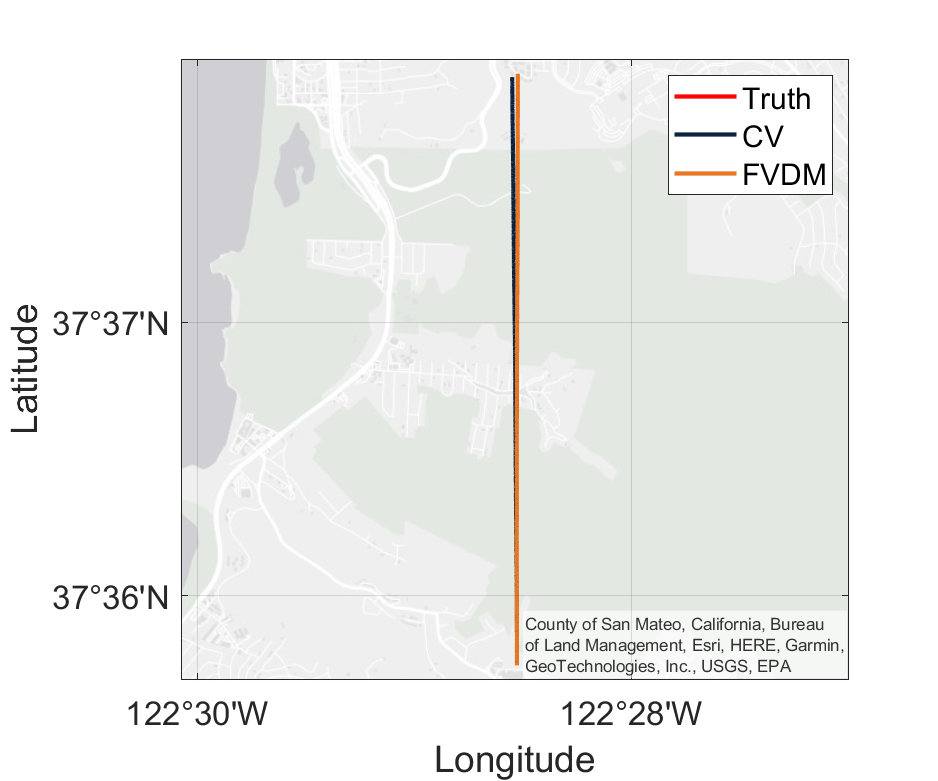
\includegraphics[width=1\linewidth]{Figures/straight/20/GEOPLOT.png}
    \end{subfigure}%
    \begin{subfigure}{.45\textwidth}
        \centering
        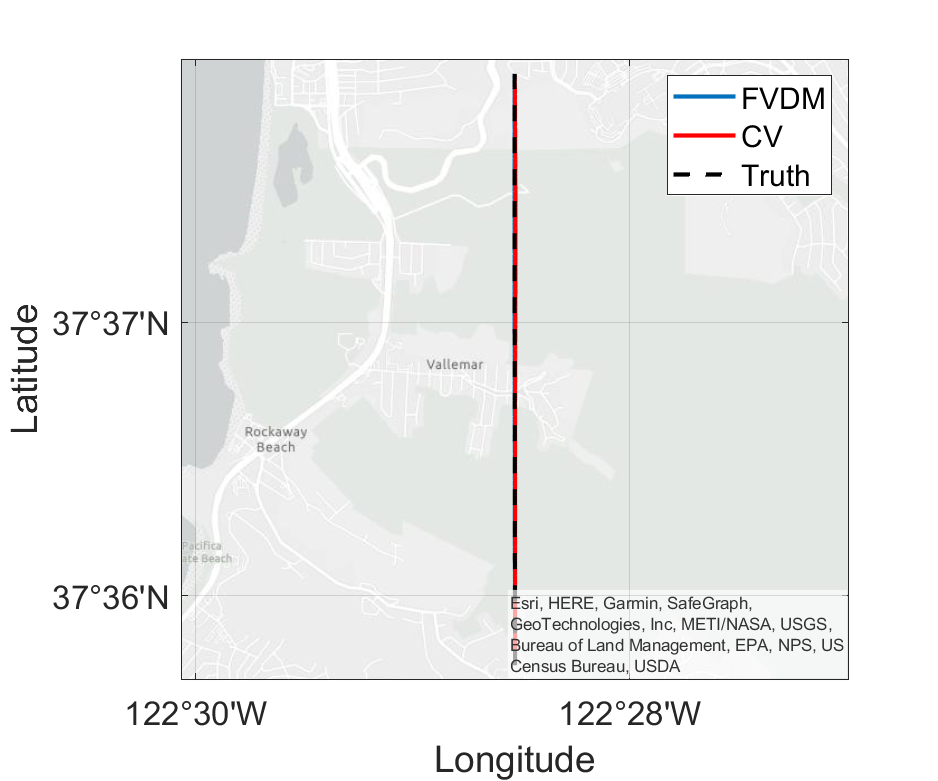
\includegraphics[width=1\linewidth]{Figures/straight/25/GEOPLOT.png}
    \end{subfigure}
    \caption{Average Latitude and Longitude of the FVDM and standard VDFLL implementation compared to the truth trajectory. The left figure is when both simulations had a signal power of \(20\) dB-Hz. The right figure is with a signal power of \(25\) dB-Hz.}\label{fig:GEOPLOT1}
\end{figure}

Even with the straight, baseline trajectory, the standard constant velocity filter begins to drift slightly when the GPS measurements are unreliable. This is partially due to the non-linear velocity at the beginning of the simulation. However, even though this is the case, the proposed navigation filter has no problem maintaining accurate tracking estimates. Based on Figure~\ref{fig:codecarrierstraight}, the deeply integrated FVDM maintains great position estimates with each channel's signal power down to \(16\) dB-Hz (Figure~\ref{fig:GEOPLOT2}). For the position estimates from the standard VDFLL implementation, the greatest error is shown in the downward direction (Figure~\ref{fig:Altitude1}).

\begin{figure}[!ht]
    \centering
    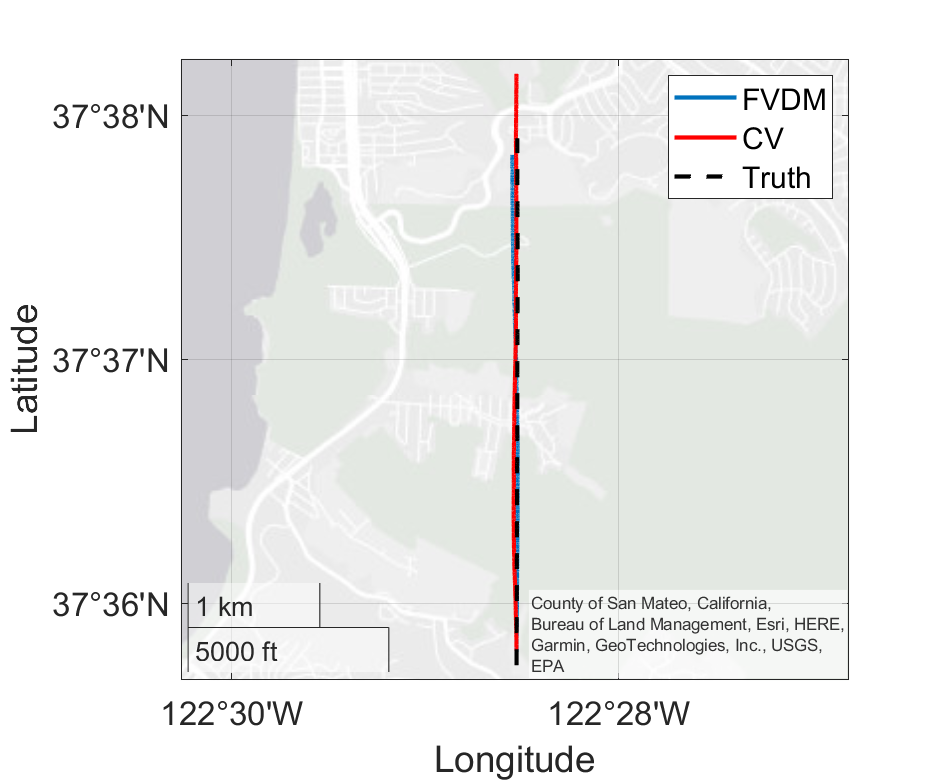
\includegraphics[width=0.5\linewidth]{Figures/straight/15/GEOPLOT.png}
    \caption{Average Latitude and Longitude of the FVDM and standard VDFLL implementation compared to the truth trajectory when subject to a degraded signal power of \(16\) dB-Hz.}\label{fig:GEOPLOT2}
\end{figure}



\begin{figure}[!ht]
    \begin{subfigure}{.45\textwidth}
        \centering
        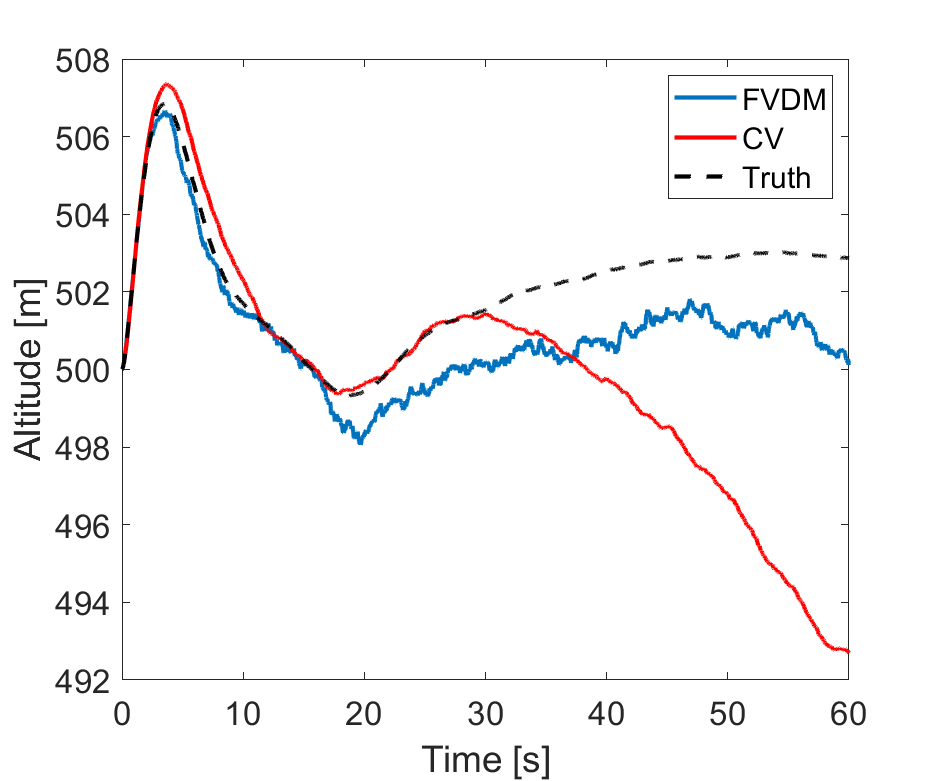
\includegraphics[width=1\linewidth]{Figures/straight/20/ALTITUDE.png}
    \end{subfigure}
    \begin{subfigure}{.45\textwidth}
        \centering
        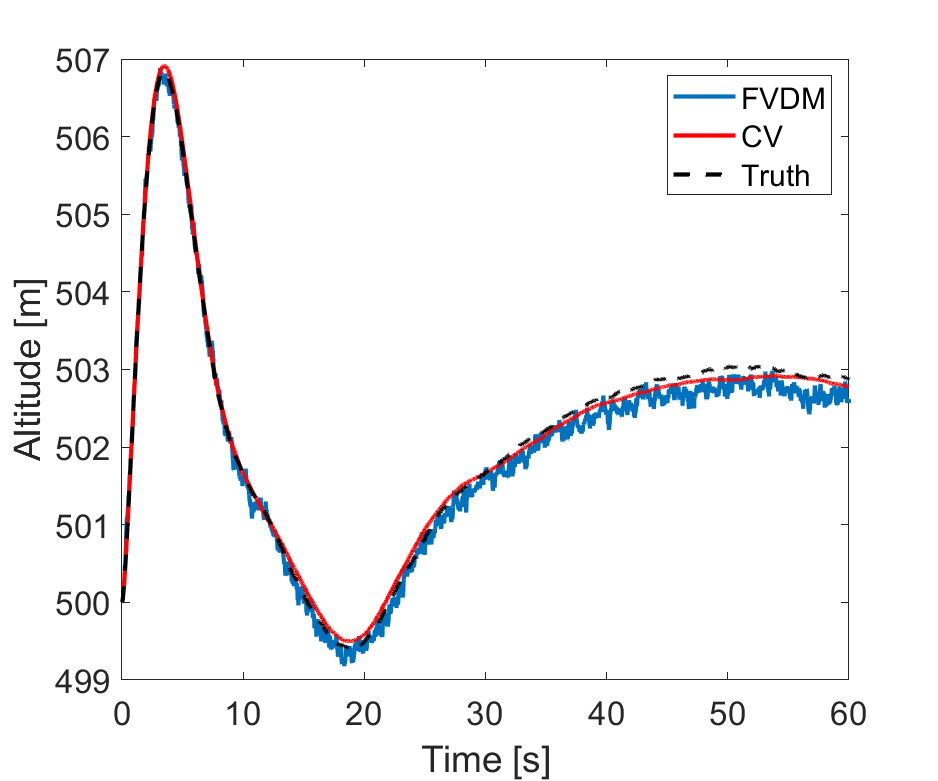
\includegraphics[width=1\linewidth]{Figures/straight/25/ALTITUDE.png}
    \end{subfigure}
    \caption{Average altitude estimates of the FVDM and standard VDFLL implementation compared to the truth trajectory. The left figure is when both simulations had a signal power of \(20\) dB-Hz. The right figure is with a signal power of \(25\) dB-Hz.}\label{fig:Altitude1}
\end{figure}

This is simply due to the lack of geometric diversity between the satellites sending the measurements. One way to solve this problem would be to include LEO satellites or signals of opportunity for improved altitude estimates from more diverse measurements. The poor assumption that the acceleration of the aircraft is zero-mean can be seen by the speed estimates in the constant-velocity kinematic model (Figure~\ref{fig:Speed1})

\begin{figure}[!ht]
    \begin{subfigure}{.45\textwidth}
        \centering
        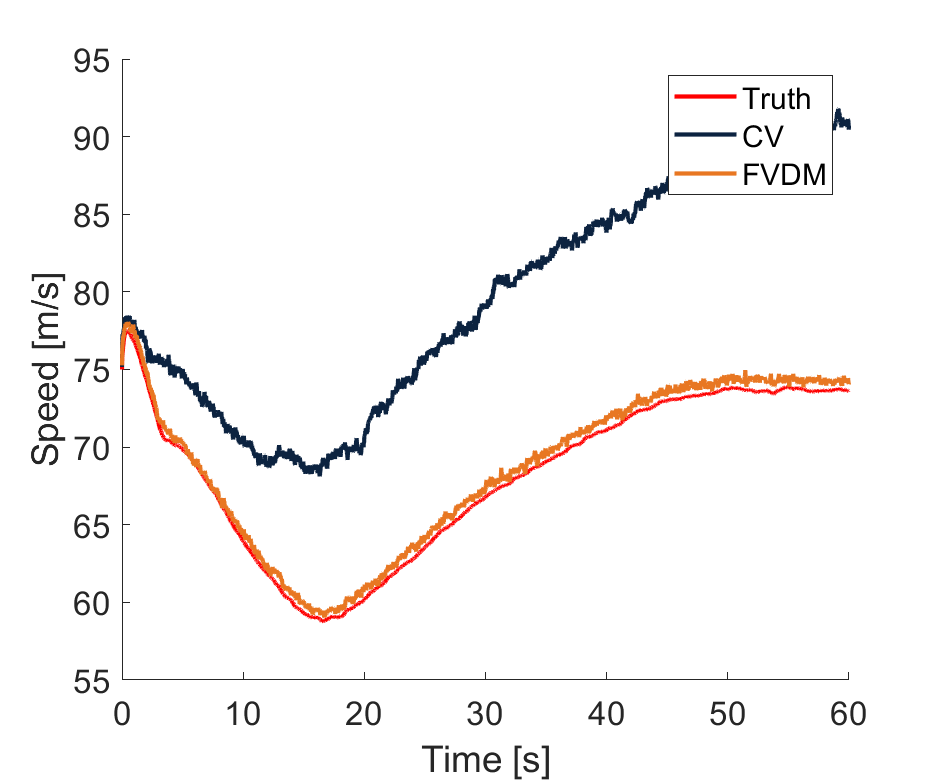
\includegraphics[width=1\linewidth]{Figures/straight/20/SPEED.png}
    \end{subfigure}
    \begin{subfigure}{.45\textwidth}
        \centering
        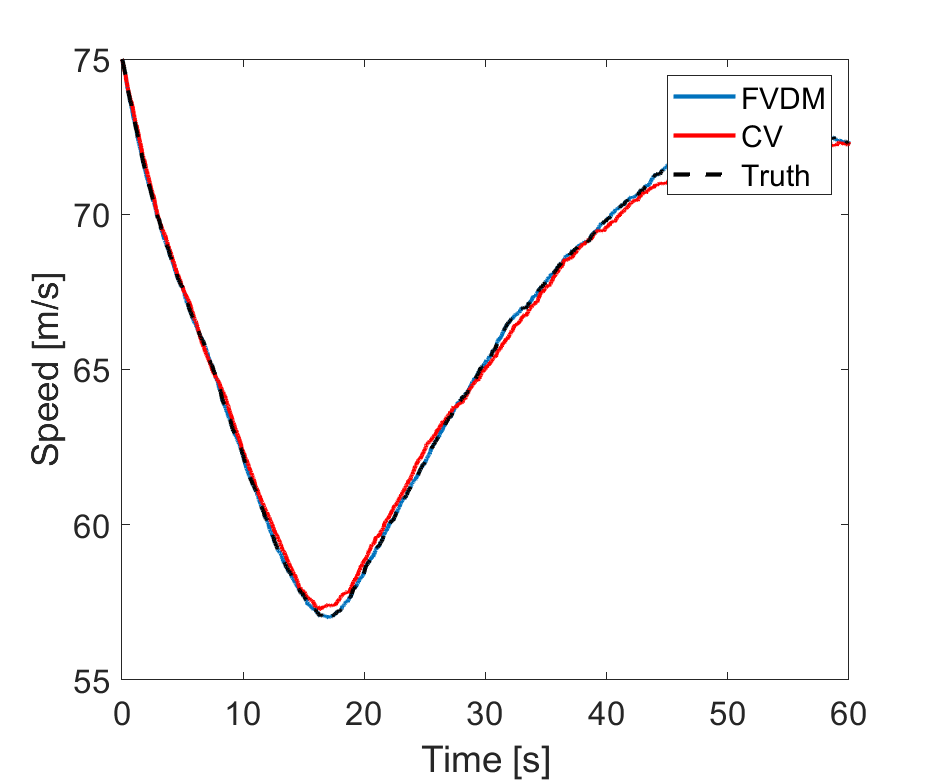
\includegraphics[width=1\linewidth]{Figures/straight/25/SPEED.png}
    \end{subfigure}
    \caption{Average speed estimates of the FVDM and standard VDFLL implementation compared to the truth trajectory. The left figure is when both simulations had a signal power of \(20\) dB-Hz. The right figure is with a signal power of \(25\) dB-Hz.}\label{fig:Speed1}
\end{figure}

When the correlator measurements from the receiver become unreliable, the constant velocity filter has no choice but to rely on its own prediction of aircraft velocity. On the fundamental basis that the velocity is the integral of a zero-mean acceleration, it leads the standard implementation to a heavily biased velocity prediction, thus deviating from the true states. Apart from the position and velocities, both filters also estimate the bias and drift of the embedded clock. As stated before, the clock used during the simulations is an OCXO\@. Figure~\ref{fig:Clocks1} presents the average clock bias estimates for each filter at both \(20\) and \(25\) dB-Hz signal power, while Figure~\ref{fig:Clocks2} presents the average clock drift estimates from each filter for the same interference cases.

\begin{figure}[!ht]
    \begin{subfigure}{.45\textwidth}
        \centering
        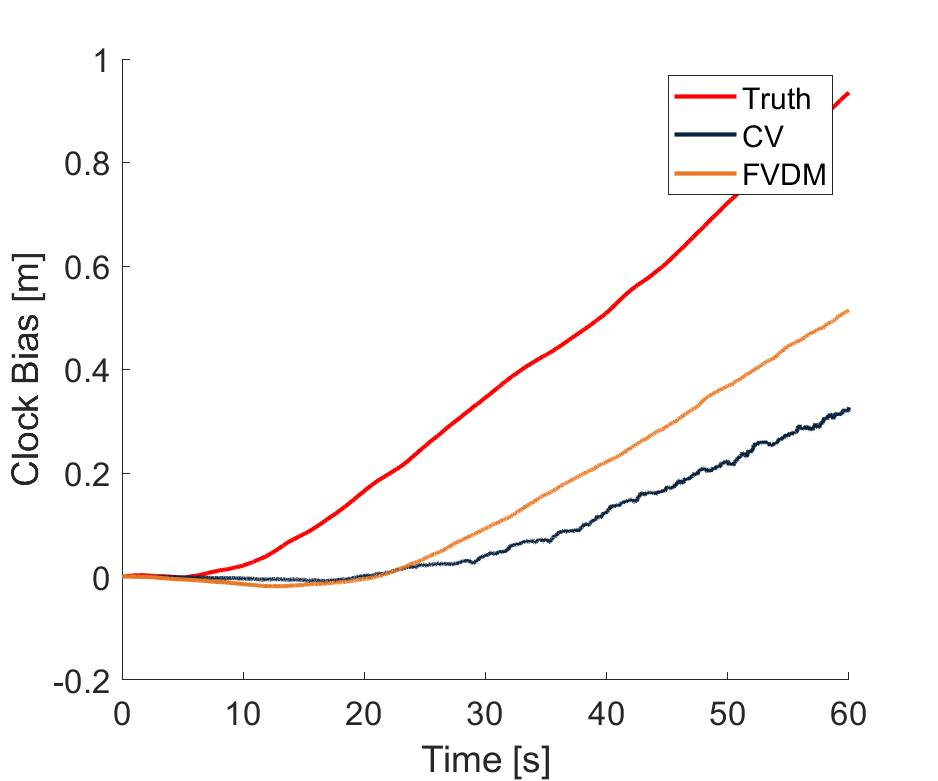
\includegraphics[width=1\linewidth]{Figures/straight/25/CLOCKBIAS.png}\
    \end{subfigure}
    \begin{subfigure}{.45\textwidth}
        \centering
        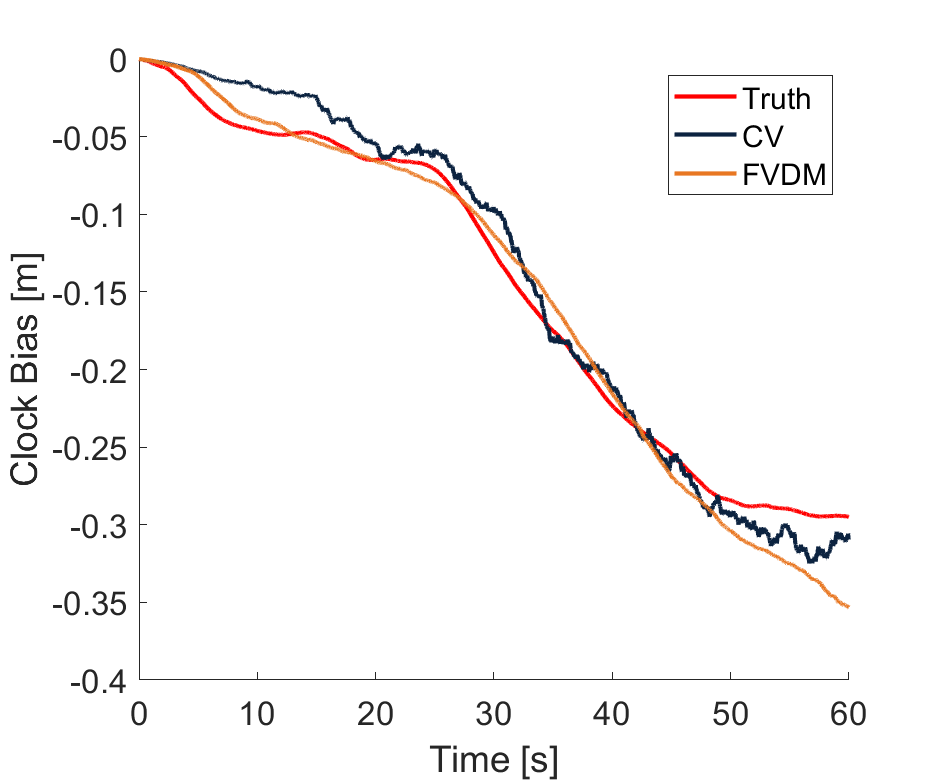
\includegraphics[width=1\linewidth]{Figures/straight/35/CLOCKBIAS.png}
    \end{subfigure}
    \caption{Average clock bias estimates of the FVDM and standard VDFLL implementation compared to the truth trajectory. The left figure is when both simulations had a signal power of \(20\) dB-Hz. The right figure is with a signal power of \(25\) dB-Hz.}\label{fig:Clocks1}
\end{figure}

\begin{figure}[!ht]
    \begin{subfigure}{.45\textwidth}
        \centering
        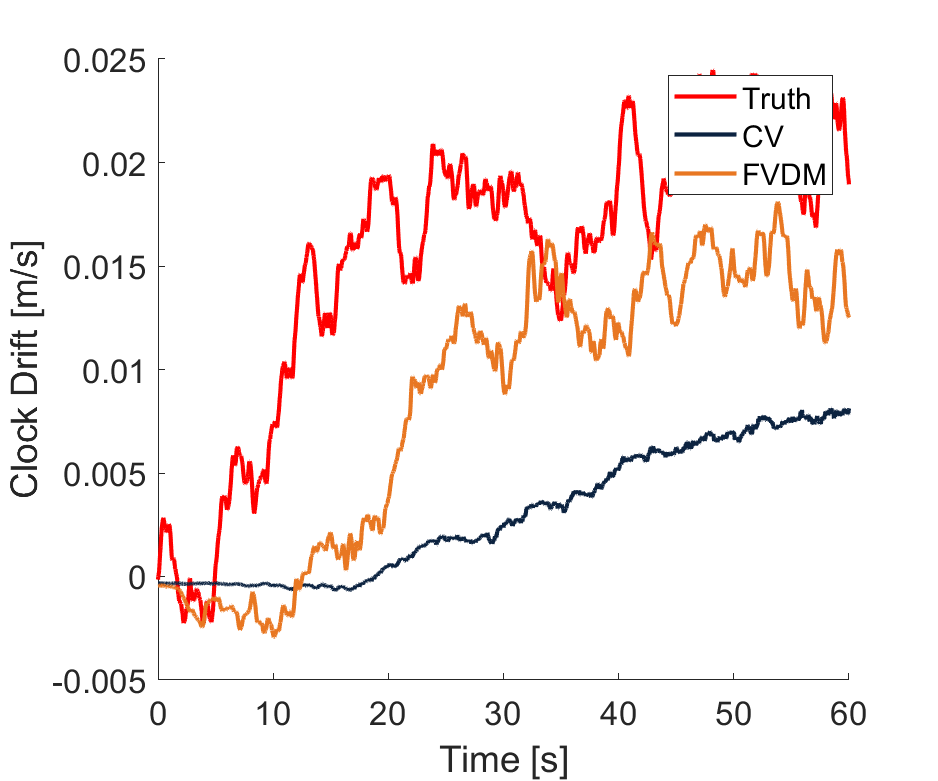
\includegraphics[width=1\linewidth]{Figures/straight/25/CLOCKDRIFT.png}\
    \end{subfigure}
    \begin{subfigure}{.45\textwidth}
        \centering
        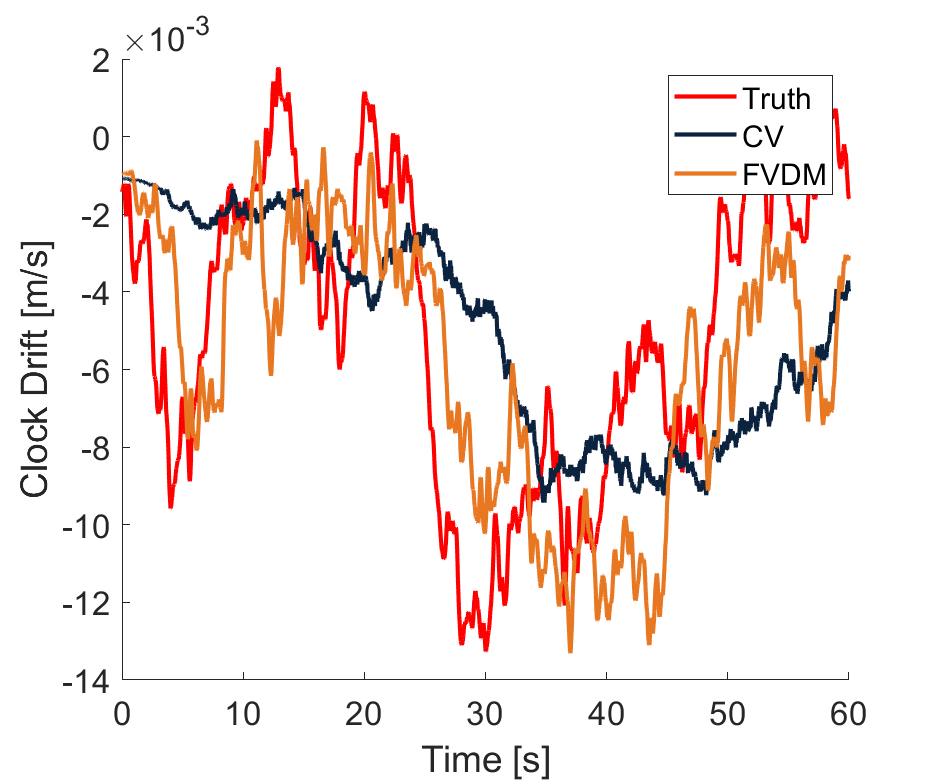
\includegraphics[width=1\linewidth]{Figures/straight/35/CLOCKDRIFT.png}
    \end{subfigure}
    \caption{Average clock drift estimates of the FVDM and standard VDFLL implementation compared to the truth trajectory. The left figure is when both simulations had a signal power of \(20\) dB-Hz. The right figure is with a signal power of \(25\) dB-Hz.}\label{fig:Clocks2}
\end{figure}

The clock model utilized from~\cite{wangKalmanFilterBasedIntegrity} is the same used on both filters, so similar performance should be expected. However, the deeply-coupled navigation filter still out performs the constant-velocity EKF in both cases. The errors in clock bias and clock drift are directly linked to position and velocity estimates seen before (Figures~\ref{fig:GEOPLOT1} and~\ref{fig:Speed1}). That is, the less error on the positional estimates means less likelihood of more error on the clock bias estimates. The same can be said for the velocity and clock drift estimates between the two filters.

As mentioned previously, the first trajectory was a baseline, litmus test where it is expected that both the proposed navigation filter and the constant velocity kinematic model would perform similarly. Regardless of the objective for the trajectory, in cases where the signal interference left the signal power to be less than \(25\) dB-Hz, the deeply-coupled FVDM begins to show improved performance. This is further illustrated by Tables~\ref{tbl:straight20FVDM} and~\ref{tbl:straight20CV} where the RMSE, STD, and maximum error found from the 100-run Monte Carlo analysis are shown for a subjected signal power of \(20\) dB-Hz.

\begin{table}[!ht]
    \caption{RMSE, STD, and maximum error from 100-run Monte Carlo simulation when the receiver is subject to a degraded signal power level of \(20\) dB-Hz.}\label{tbl:straight20FVDM}
    \centering
    \begin{tabular}{ccccc}
        \toprule
                  & Position [m] & Speed [m/s] & Clock Bias [m] & Clock Drift [m/s] \\
        \midrule
        RMSE      & 0.83733      & 0.27649     & 0.14072        & 0.0087105         \\
        STD       & 0.32434      & 0.13394     & 0.13147        & 0.0072989         \\
        Max Error & 1.8783       & 0.90375     & 0.48541        & 0.024451          \\
        \bottomrule
    \end{tabular}
\end{table}

\begin{table}[!ht]
    \caption{RMSE, STD, and maximum error from 100-run Monte Carlo simulation when the receiver is subject to a degraded signal power level of \(20\) dB-Hz.}\label{tbl:straight20CV}
    \centering
    \begin{tabular}{ccccc}
        \toprule
                  & Position [m] & Speed [m/s] & Clock Bias [m] & Clock Drift [m/s] \\
        \midrule
        RMSE      & 24.567       & 0.88208     & 0.17748        & 0.0088036         \\
        STD       & 10.287       & 0.34973     & 0.14068        & 0.005286          \\
        Max Error & 36.193       & 2.0585      & 0.50134        & 0.022316          \\
        \bottomrule
    \end{tabular}
\end{table}

\section{\textbf{Second Trajectory}}
For the second trajectory, the aircraft is simulated for a more dynamic flight pattern while commanded to climb to an altitude of 1150 meters above sea level (Figure~\ref{fig:trajectory2}). The dynamics induced by trajectory two show the effectiveness of the deeply-coupled FVDM to predict the behavior of the aircraft due to the additional angular rates and Euler attitude being estimated. It is assumed that the receiver knows it position beforehand when the simulation begins. Similarly to the first trajectory, the receiver aboard the aircraft is subject to seven different cases of interference that degrade the signals from the nine tracked channels (Table~\ref{tbl:interferenceCases}). The receiver is subject to these degraded power levels for the entirety of the 60 second simulation.

\begin{figure}[!ht]
    \centering
    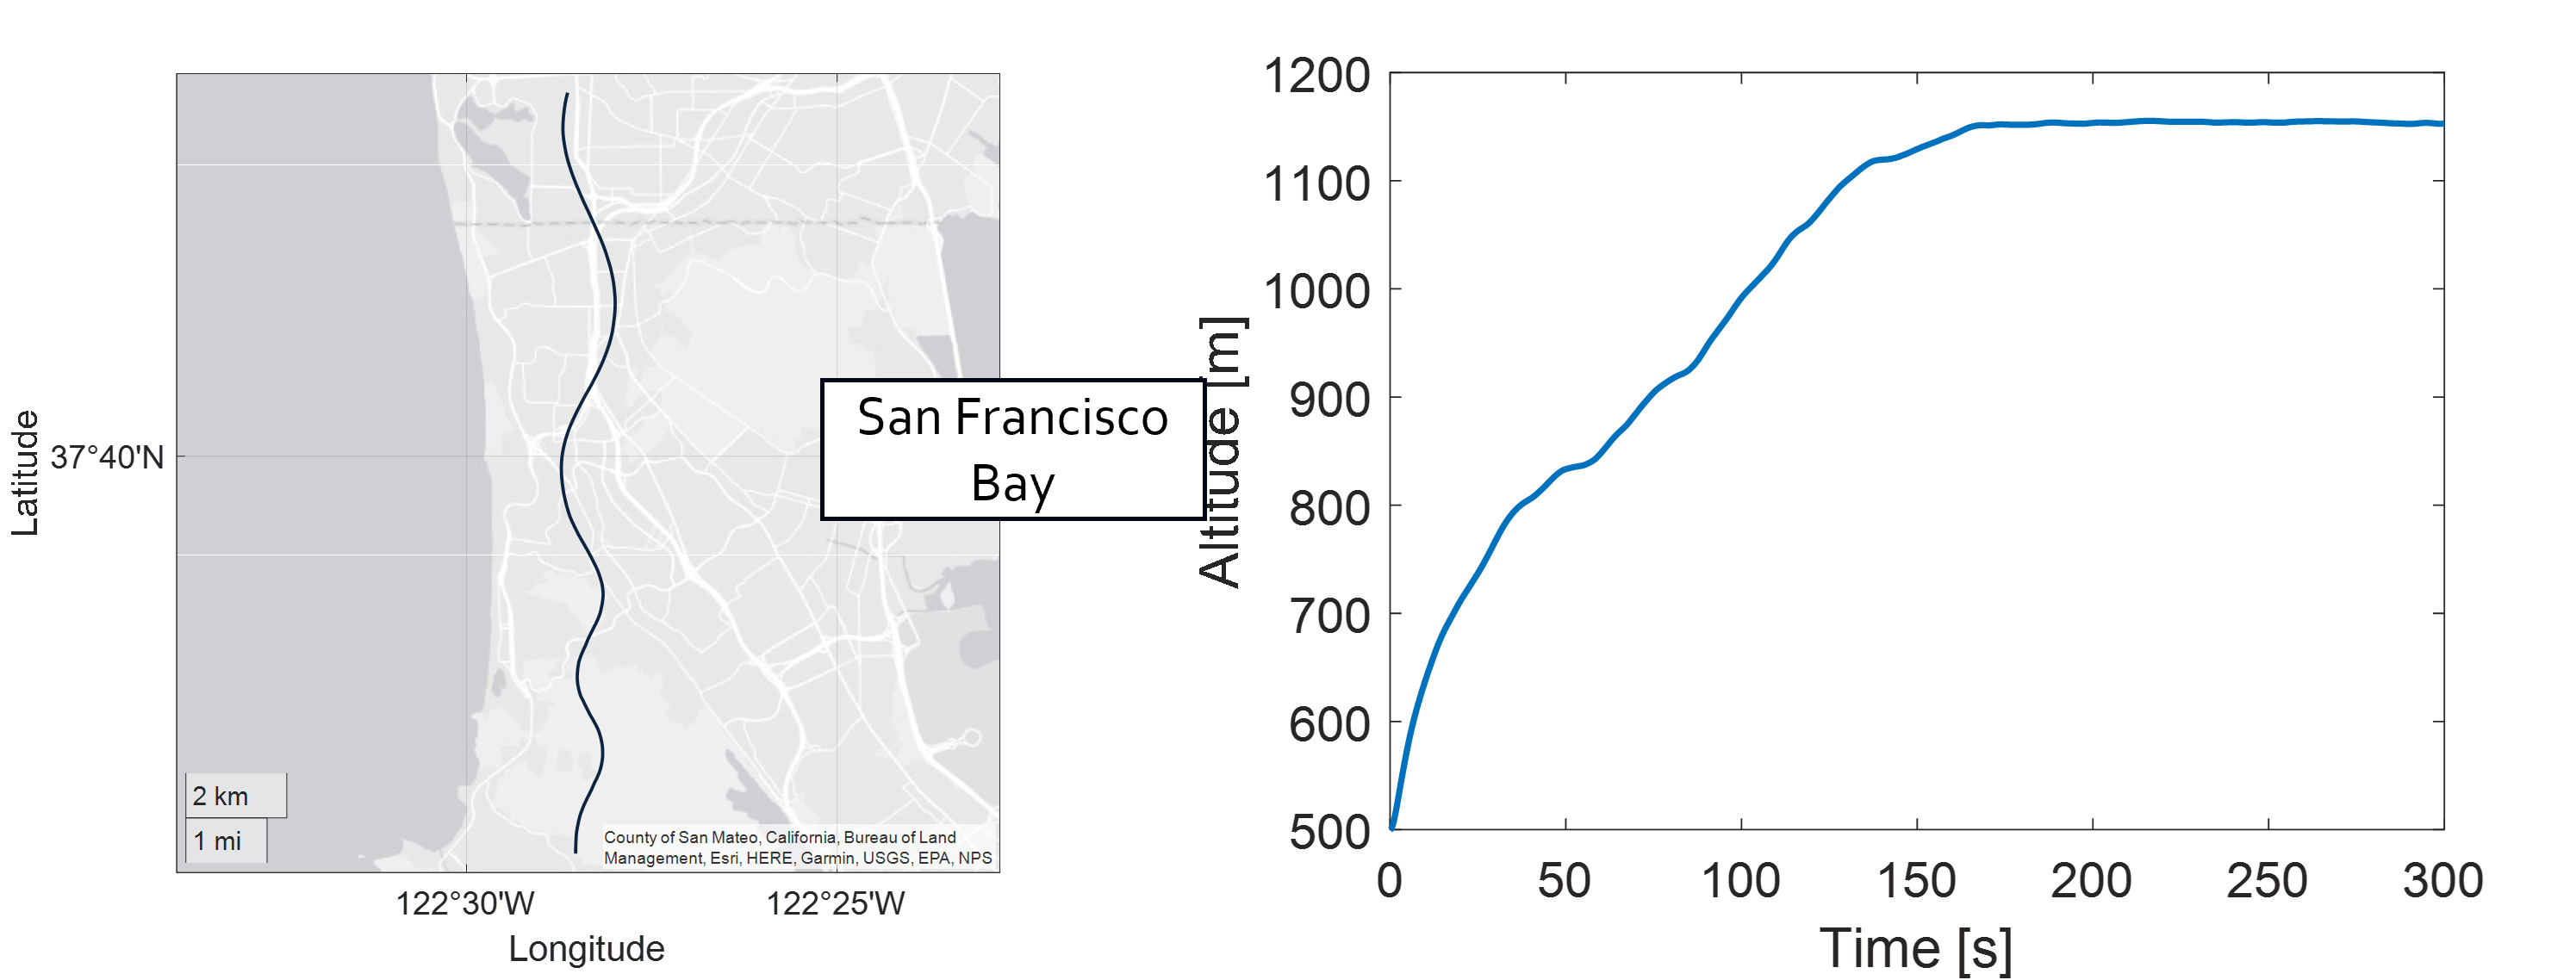
\includegraphics[width=\linewidth]{Figures/Results/trajectory2.png}
    \caption{(Left) Top-view of simulated flight path for the second trajectory. (Right) Altitude of second flight path where aircraft is commanded to climb to 1150 meters and then maintain the altitude for the remainder of the simulation.}\label{fig:trajectory2}
\end{figure}

It should be noted that the same cases of interference from the first trajectory still apply to trajectory two (Table~\ref{tbl:interferenceCases}). Furthermore, the only change in configuration between the first and second trajectory is the specified flight path. For this dynamic trajectory, \textit{SCurveFlightPath.mat} will be used in place of the \textit{StraightFlightPath.mat} used previously. The satellites found in-view utilizing the broadcast ephemeris file for the specified date are the same satellites used during the following simulations (Figure~\ref{fig:skyplot}). One of the benefits (on top of improved estimate performance) of utilizing the deeply-coupled FVDM is the capability to estimate the attitude and attitude rate of the aircraft during flight. This can be imperative for acrobatic or urban air mobility aircraft that roll, pitch, and yaw as their nominal flight motion. Similar to IMU and other hardware sensors, the excitation caused by the rolling and pitching motion of aircraft for trajectory two is expected to increase the performance of the position and velocity estimates along with the capability to maintain channel lock at heavier signal degradation.

\subsection{\textbf{Monte-Carlo Analyses}}
From Monte-Carlo results, several parameters can analyzed for the performance improvements of the proposed navigation filter over the standard VDFLL kinematic model. This section begins with an analysis of the signal-level results between the two filters and follows with an analysis of the state estimate performance for a range of \(C/N_0\) values. For the range of signal interference presented in table~\ref{tbl:interferenceCases}, the RMSE of both the code phase and carrier frequency shows improved performance by using the deeply-coupled FVDM in GPS-challenged environments (Figure~\ref{fig:codecarrierdyn}).

\begin{figure}[!ht]
    \begin{subfigure}{.45\textwidth}
        \centering
        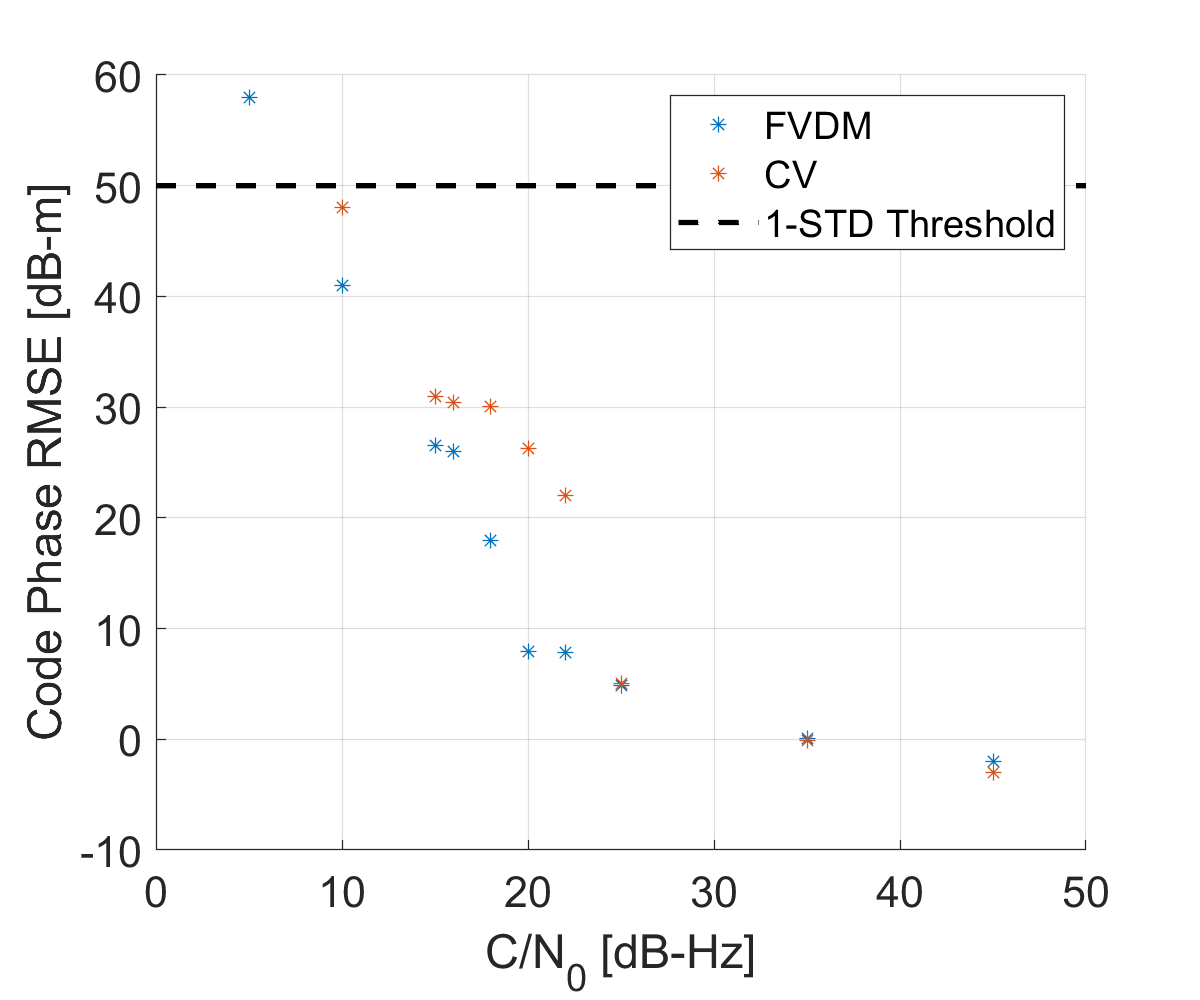
\includegraphics[width=1\linewidth]{Figures/dynamic/codephaseRMSEdyn.png}
    \end{subfigure}%
    \begin{subfigure}{.45\textwidth}
        \centering
        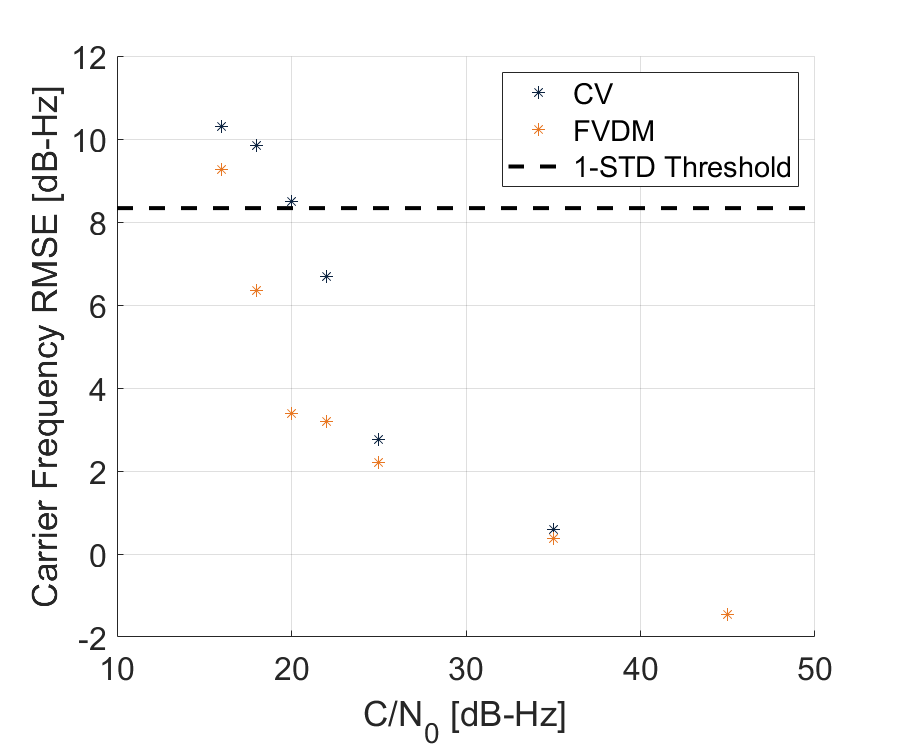
\includegraphics[width=1\linewidth]{Figures/dynamic/carrFreqRMSEdyn.png}
    \end{subfigure}
    \caption{Code phase and carrier frequency RMSE as a function of signal power, specified in dB-Hz.}\label{fig:codecarrierdyn}
\end{figure}

As previously mentioned, the excitation in the angular rates provides better observability for those estimated states along with their integrated Euler attitude counter parts. Compared to trajectory one, Figure~\ref{fig:codecarrierdyn} shows that the proposed navigation filter can track beyond \(16\) dB-Hz. Unlike the previous trajectory, even in cases of little to no interference, the deeply-coupled FVDM out performs the standard VDFLL implementation right up to benign signal power (\(45\) dB-Hz). This effective increase in performance is further shown in Figure~\ref{fig:trackingprobability2} where the probability to maintain lock across all channels is shown again for trajectory two.

\begin{figure}[!ht]
    \centering
    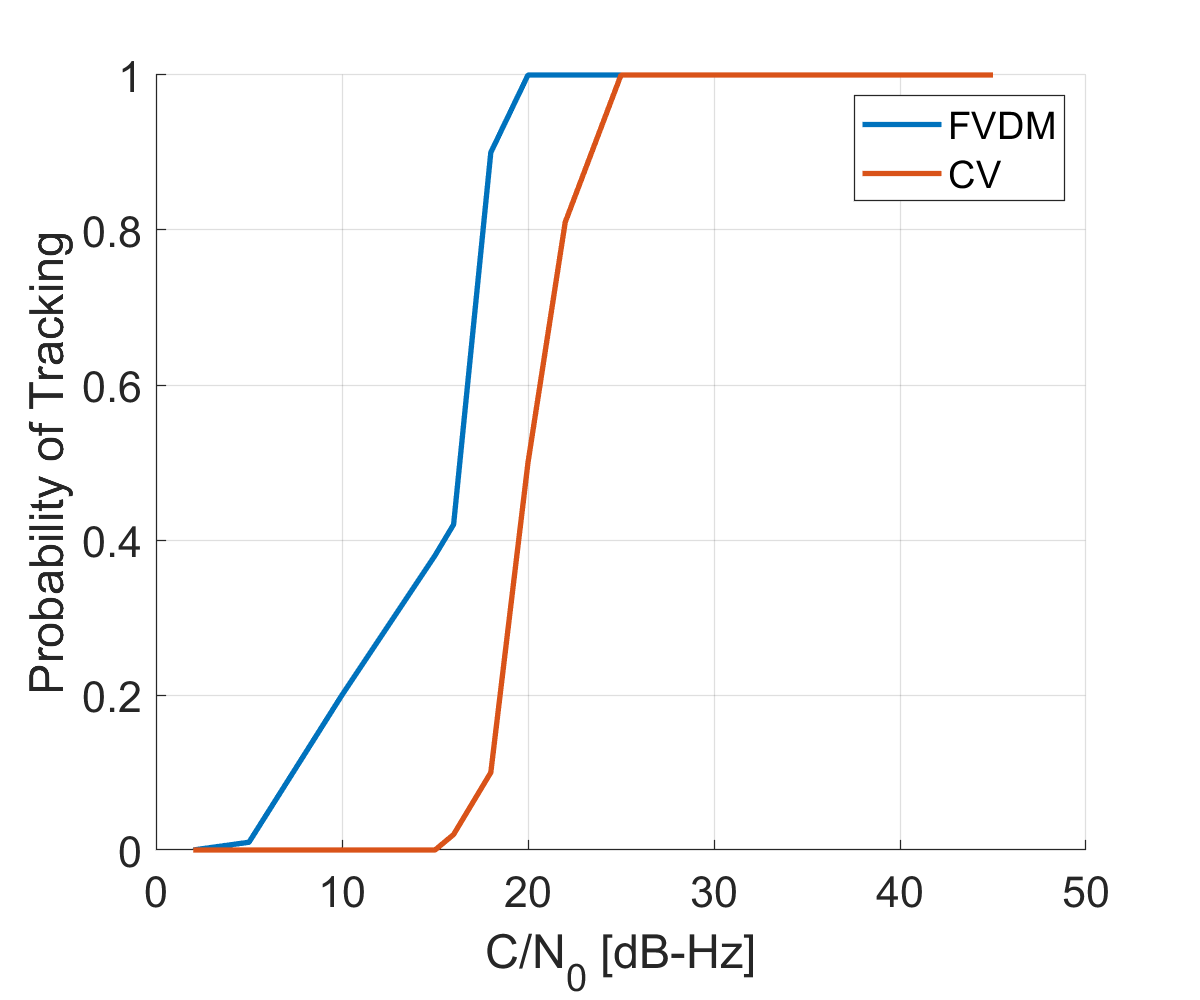
\includegraphics[width=0.5\linewidth]{Figures/dynamic/trackingprobdyn.png}
    \caption{The probability that each navigation filter is able to maintain channel lock throughout the simulation across different levels of signal interference.}\label{fig:trackingprobability2}
\end{figure}

While the deeply integrated FVDM shows approximately \(100\% \) tracking probability at the same \(20\) dB-Hz compared to Figure~\ref{fig:trackingprobability1}, the constant velocity kinematic model effectively loses lock faster after the the signal power drops below \(25\) dB-Hz. Similar to trajectory one, the same \(5\) dB-Hz improvement in tracking probability can be seen for trajectory two. The position estimates reflect the improved ability of the deeply-coupled FVDM to maintain lock in GPS-challenged environments. Figure~\ref{fig:GEOPLOT3} presents the Latitude and Longitude estimates for both filters simulated for trajectory two.

\begin{figure}[!ht]
    \begin{subfigure}{.45\textwidth}
        \centering
        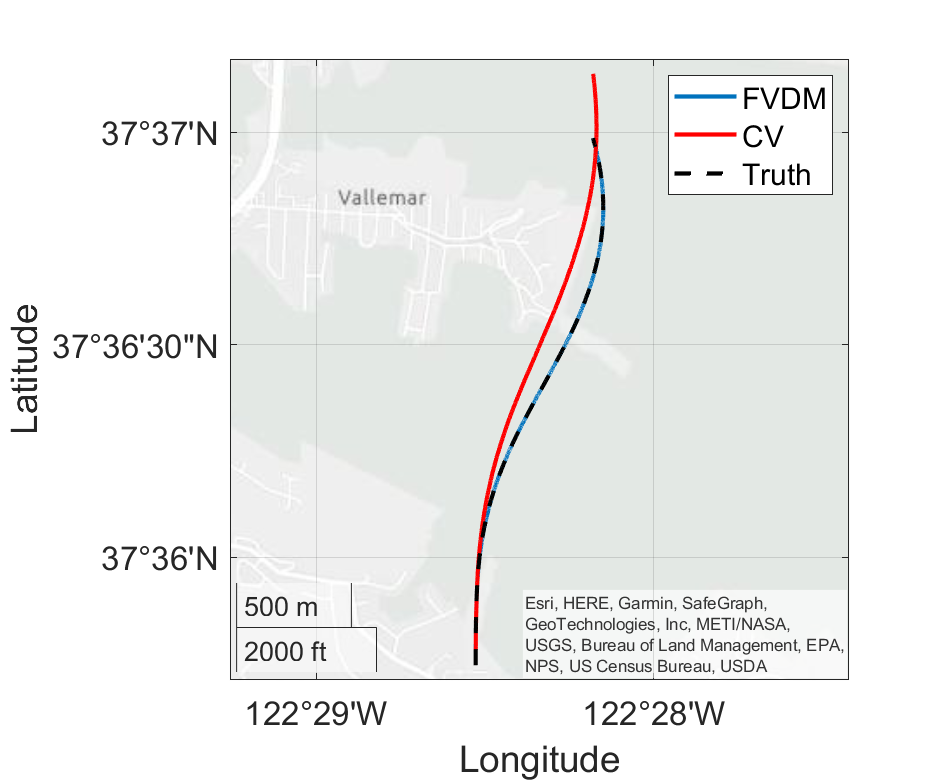
\includegraphics[width=1\linewidth]{Figures/dynamic/20/GEOPLOT.png}
    \end{subfigure}%
    \begin{subfigure}{.45\textwidth}
        \centering
        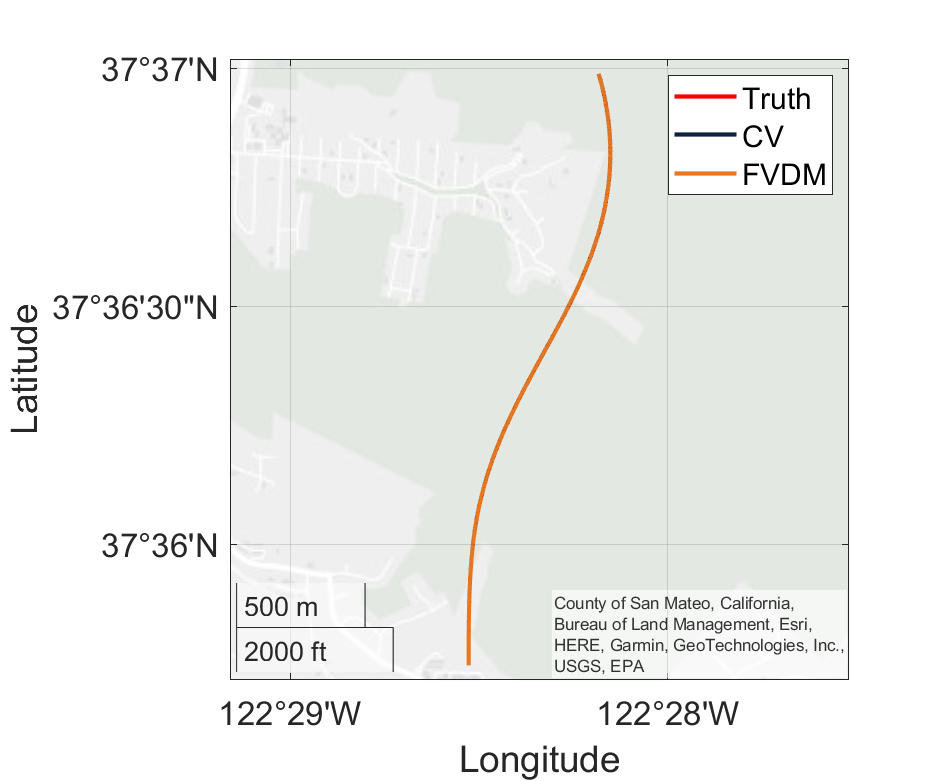
\includegraphics[width=1\linewidth]{Figures/dynamic/25/GEOPLOT.png}
    \end{subfigure}
    \caption{Average Latitude and Longitude of the FVDM and standard VDFLL implementation compared to the truth trajectory. The left figure is when both simulations had a signal power of \(20\) dB-Hz. The right figure is with a signal power of \(25\) dB-Hz.}\label{fig:GEOPLOT3}
\end{figure}

When subject to a signal power of \(20\) dB-Hz, the average Latitude and Longitude estimates for the constant velocity EKF shows a slight drift from the true location of the aircraft. Like before, this is likely due to the zero-mean acceleration assumption of the kinematic model. Furthermore, the standard VDFLL implementation is unable to predict the attitude of the aircraft, making it unable to correlate velocity and Euler attitude errors. For consistency, Figure~\ref{fig:GEOPLOT4} shows the Latitude and Longitude estimates when the receiver is subject to a signal power of \(18\) dB-Hz.

\begin{figure}[!ht]
    \centering
    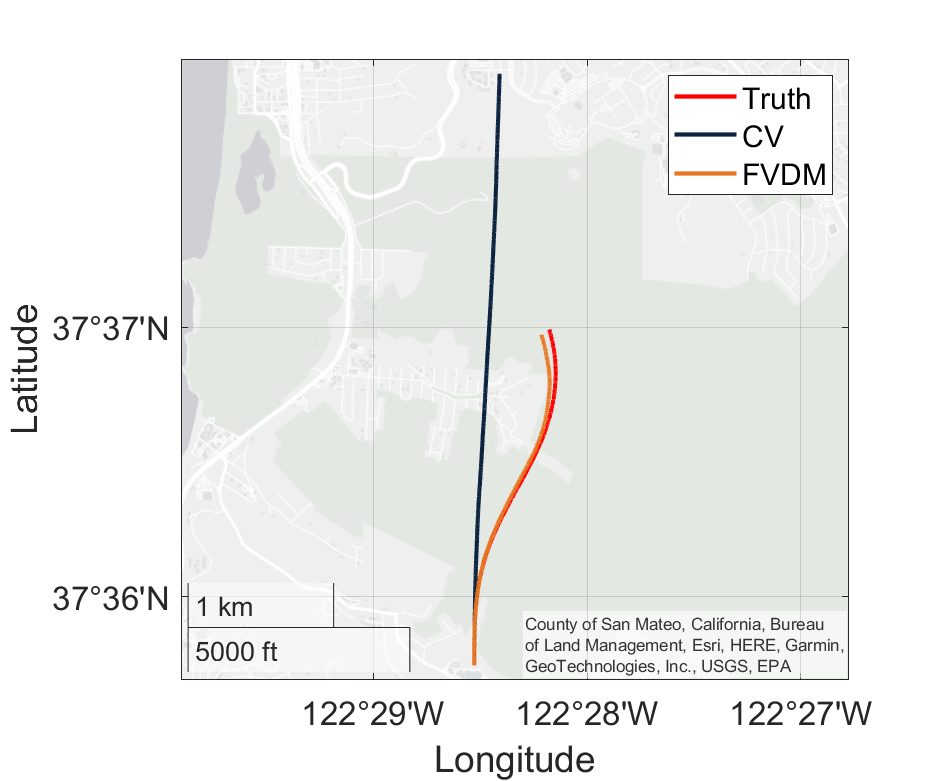
\includegraphics[width=0.5\linewidth]{Figures/dynamic/18/GEOPLOT.png}
    \caption{Average Latitude and Longitude of the FVDM and standard VDFLL implementation compared to the truth trajectory when subject to a degraded signal power of \(16\) dB-Hz.}\label{fig:GEOPLOT4}
\end{figure}

At this level of interference, it is clear the constant velocity EKF faults just after initialization. With the lack of GPS correlator measurements to make corrections, the predicted location of aircraft quickly falls off target. The excited pitching motion of the aircraft brings about an improvement on the altitude estimates of the aircraft during the simulation (Figure~\ref{fig:Altitude2}).

\begin{figure}[!ht]
    \begin{subfigure}{.45\textwidth}
        \centering
        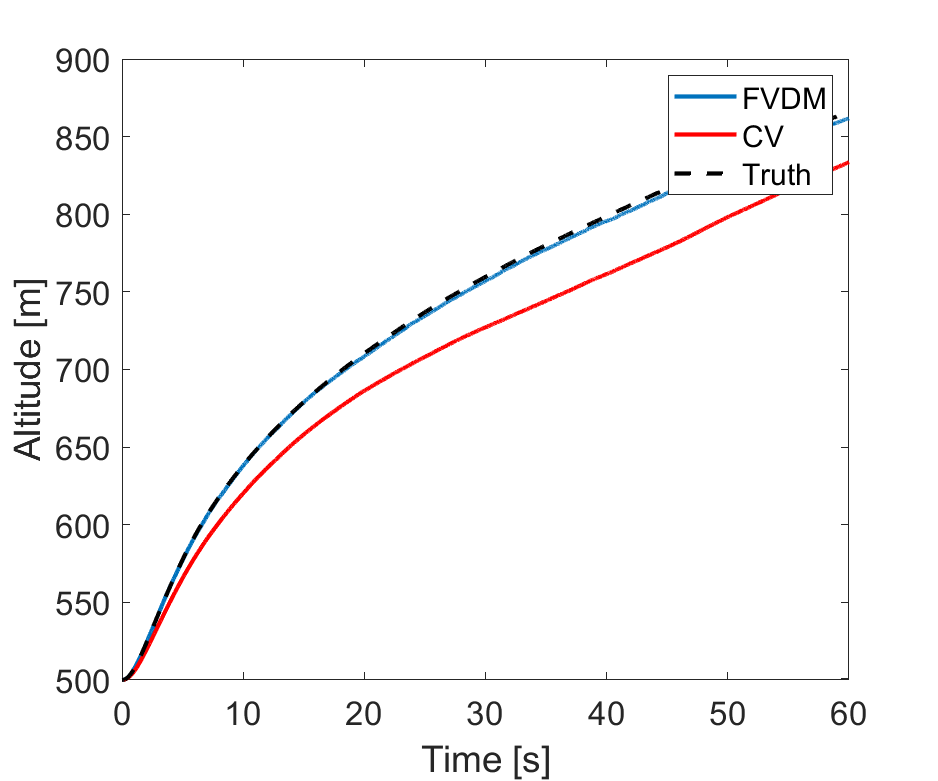
\includegraphics[width=1\linewidth]{Figures/dynamic/20/ALTITUDE.png}
    \end{subfigure}
    \begin{subfigure}{.45\textwidth}
        \centering
        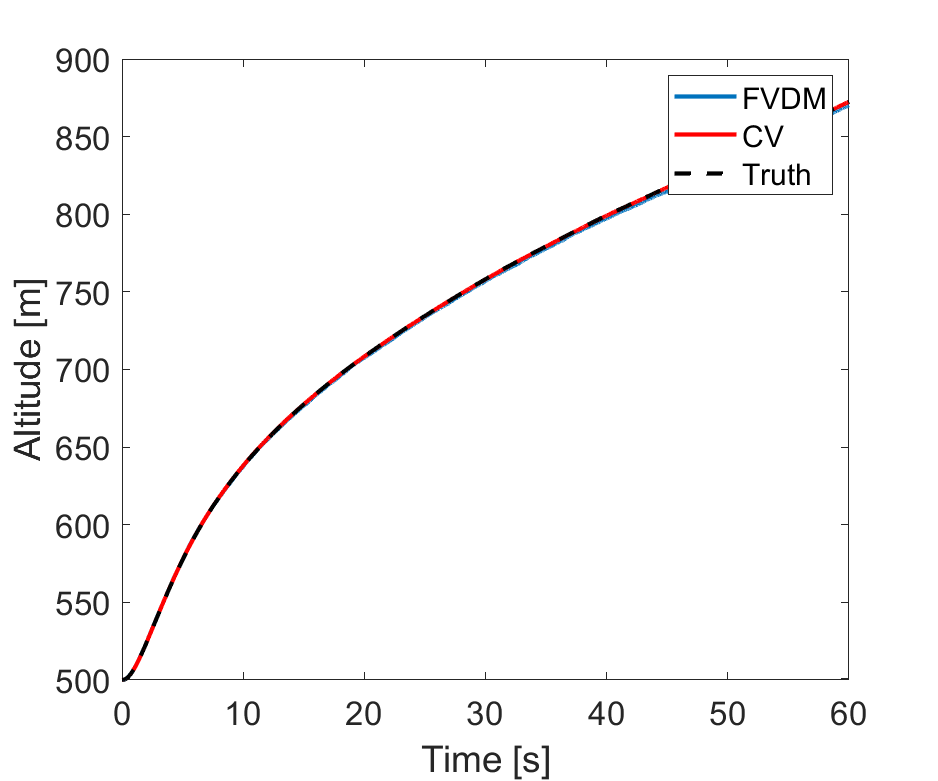
\includegraphics[width=1\linewidth]{Figures/dynamic/25/ALTITUDE.png}
    \end{subfigure}
    \caption{Average altitude estimates of the FVDM and standard VDFLL implementation compared to the truth trajectory. The left figure is when both simulations had a signal power of \(20\) dB-Hz. The right figure is with a signal power of \(25\) dB-Hz.}\label{fig:Altitude2}
\end{figure}

Again, the standard VDFLL implementation shows altitude errors of roughly \(65\) meters when provided with unreliable GPS correlator measurements. The lack of diversity is to blame and adding a ground station or fusing the solution with a external sensor or FVDM would mitigate this problem. For a more detailed reference on the difference in pose estimates between the two filters, Tables~\ref{tbl:dyn20CV} and~\ref{tbl:dyn20FVDM} are included at the end of this section for further inspection. The dynamics of trajectory two prove ever more that the zero-acceleration assumption from the constant velocity kinematic model is poor. Figure~\ref{fig:Speed2} presents the speed estimates of both the proposed navigation filter and the standard VDFLL implementation subject to \(20\) and \(25\) dB-Hz of signal power.

\begin{figure}[!ht]
    \begin{subfigure}{.45\textwidth}
        \centering
        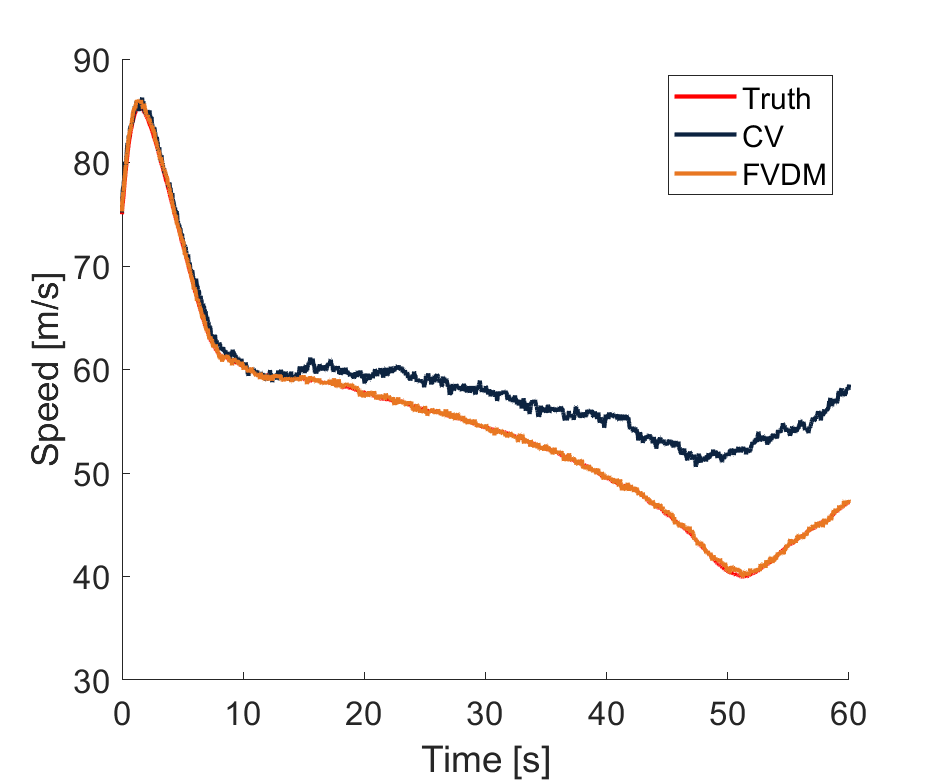
\includegraphics[width=1\linewidth]{Figures/dynamic/20/SPEED.png}
    \end{subfigure}
    \begin{subfigure}{.45\textwidth}
        \centering
        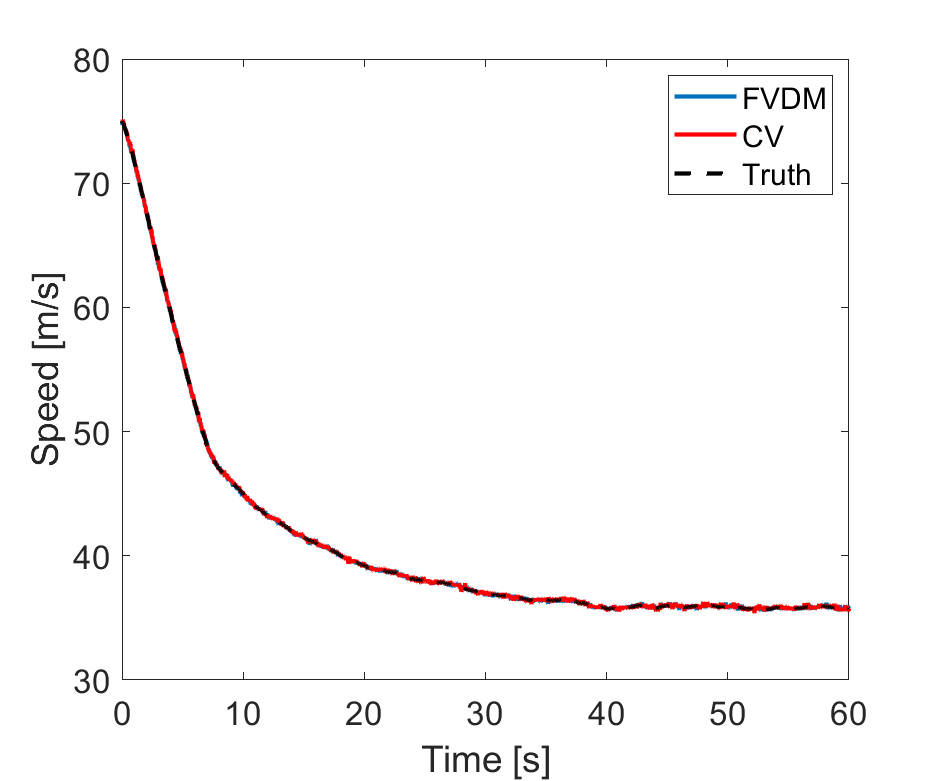
\includegraphics[width=1\linewidth]{Figures/dynamic/25/SPEED.png}
    \end{subfigure}
    \caption{Average speed estimates of the FVDM and standard VDFLL implementation compared to the truth trajectory. The left figure is when both simulations had a signal power of \(20\) dB-Hz. The right figure is with a signal power of \(25\) dB-Hz.}\label{fig:Speed2}
\end{figure}

At roughly \(10~m/s\) of error in the speed estimate (according to Table~\ref{tbl:dyn20CV}), The average drift of the estimated position presented by Figure~\ref{fig:GEOPLOT4} is understandable. It should be noted here that the throttle reference command (Chapter 5) is commanding the aircraft to keep a consistent velocity of \(70~m/s\), limitations on engine power and the advance ratio of the propeller prevent it from reaching such speeds during the climb segment. One of the primary benefits of the proposed navigation filter is the ability to estimate the angular rates and Euler attitude of the aircraft during flight. Although these states are not directly measurable by the correlator measurements, their correlation within the position and velocity equations (Equations~\ref{eq:posrate} and~\ref{eq:acc}) is substantial enough to hold accurate estimates (Figure~\ref{fig:ANGRATES}).

\begin{figure}[!ht]
    \begin{subfigure}{.45\textwidth}
        \centering
        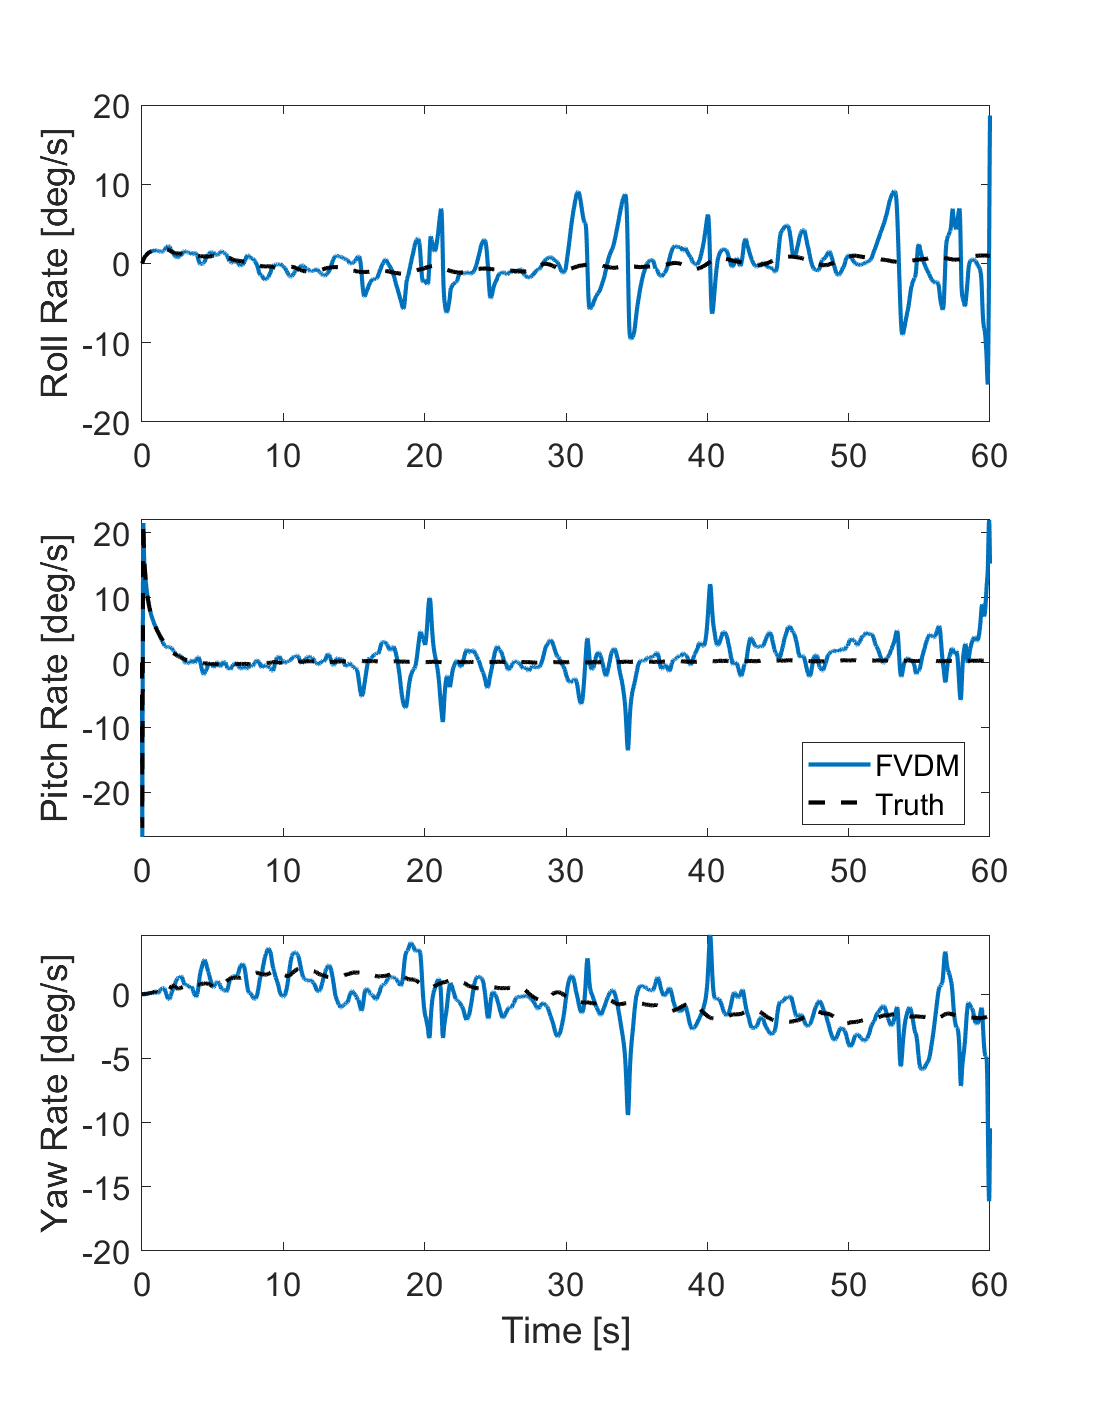
\includegraphics[width=1\linewidth]{Figures/dynamic/15/ANGULARRATES.png}
    \end{subfigure}
    \begin{subfigure}{.45\textwidth}
        \centering
        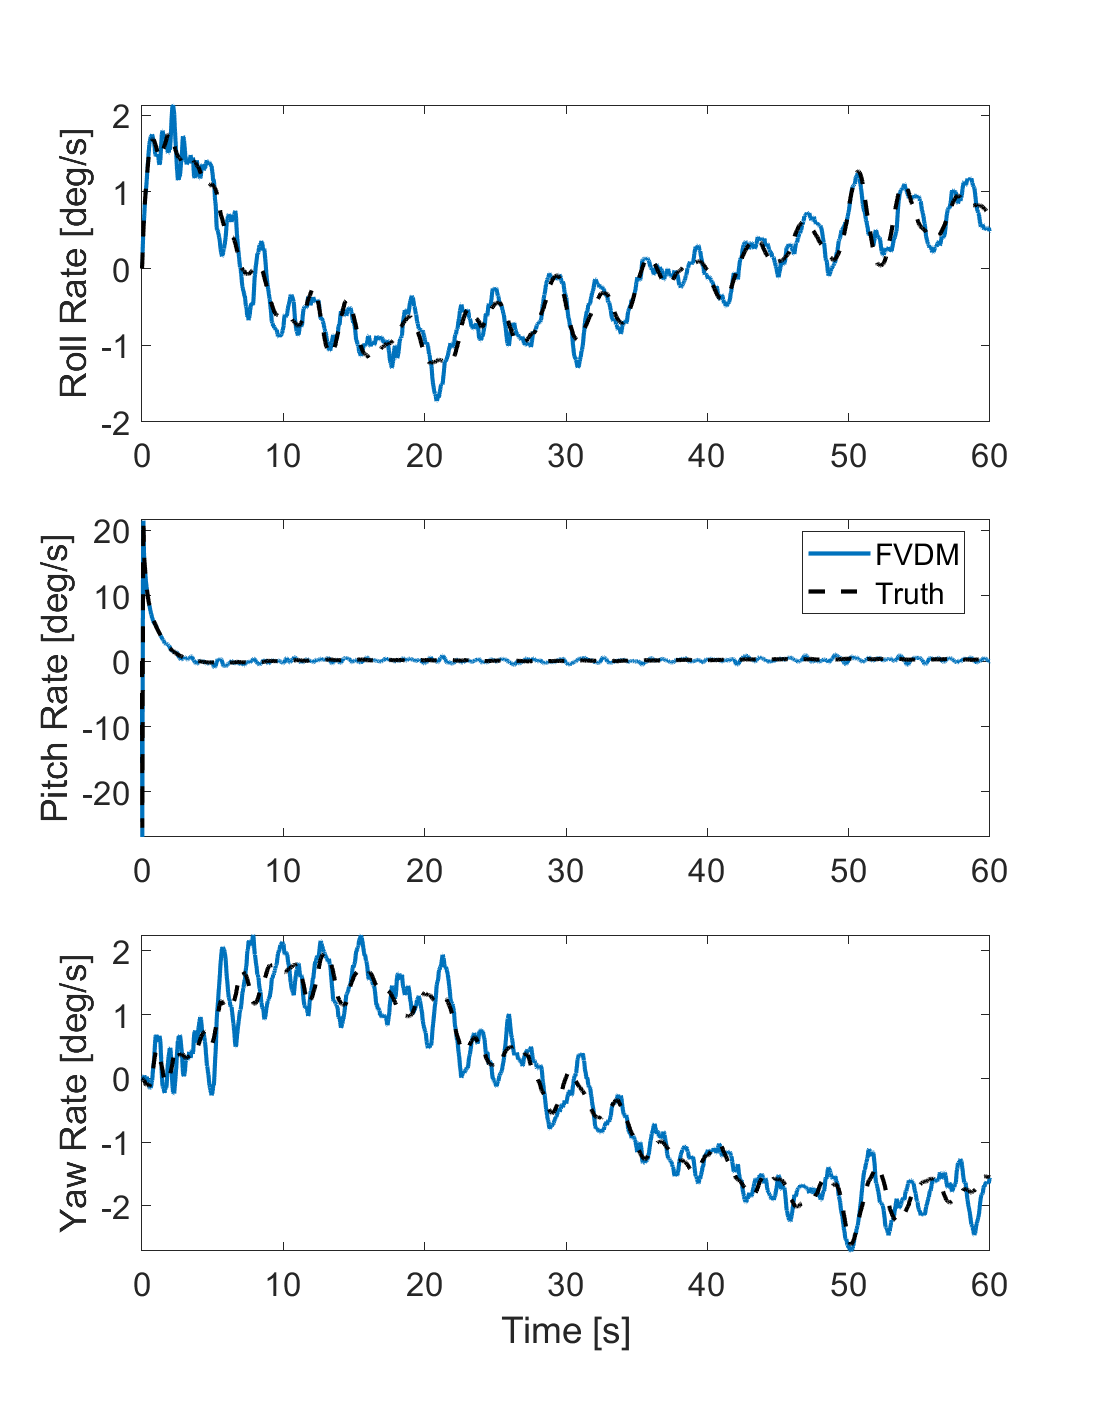
\includegraphics[width=1\linewidth]{Figures/dynamic/20/ANGULARRATES.png}
    \end{subfigure}
    \caption{Average angular rate estimates of the FVDM and standard VDFLL implementation compared to the truth trajectory. The left figure is when both simulations had a signal power of \(15\) dB-Hz. The right figure is with a signal power of \(20\) dB-Hz.}\label{fig:ANGRATES}
\end{figure}

Although the aircraft is commanded to reach an altitude of \(1150\) meters above sea level, this does not equate to radical change in pitch rate. As seen from Figure~\ref{fig:EULER}, the aircraft reaches a steady state pitch and maintains that pitch until the altitude command is met. Since the pitch command is near-constant, unlike the roll and yaw angles, leaves the pitch rate to be near-zero for the duration of the simulation.

\begin{figure}[!ht]
    \begin{subfigure}{.45\textwidth}
        \centering
        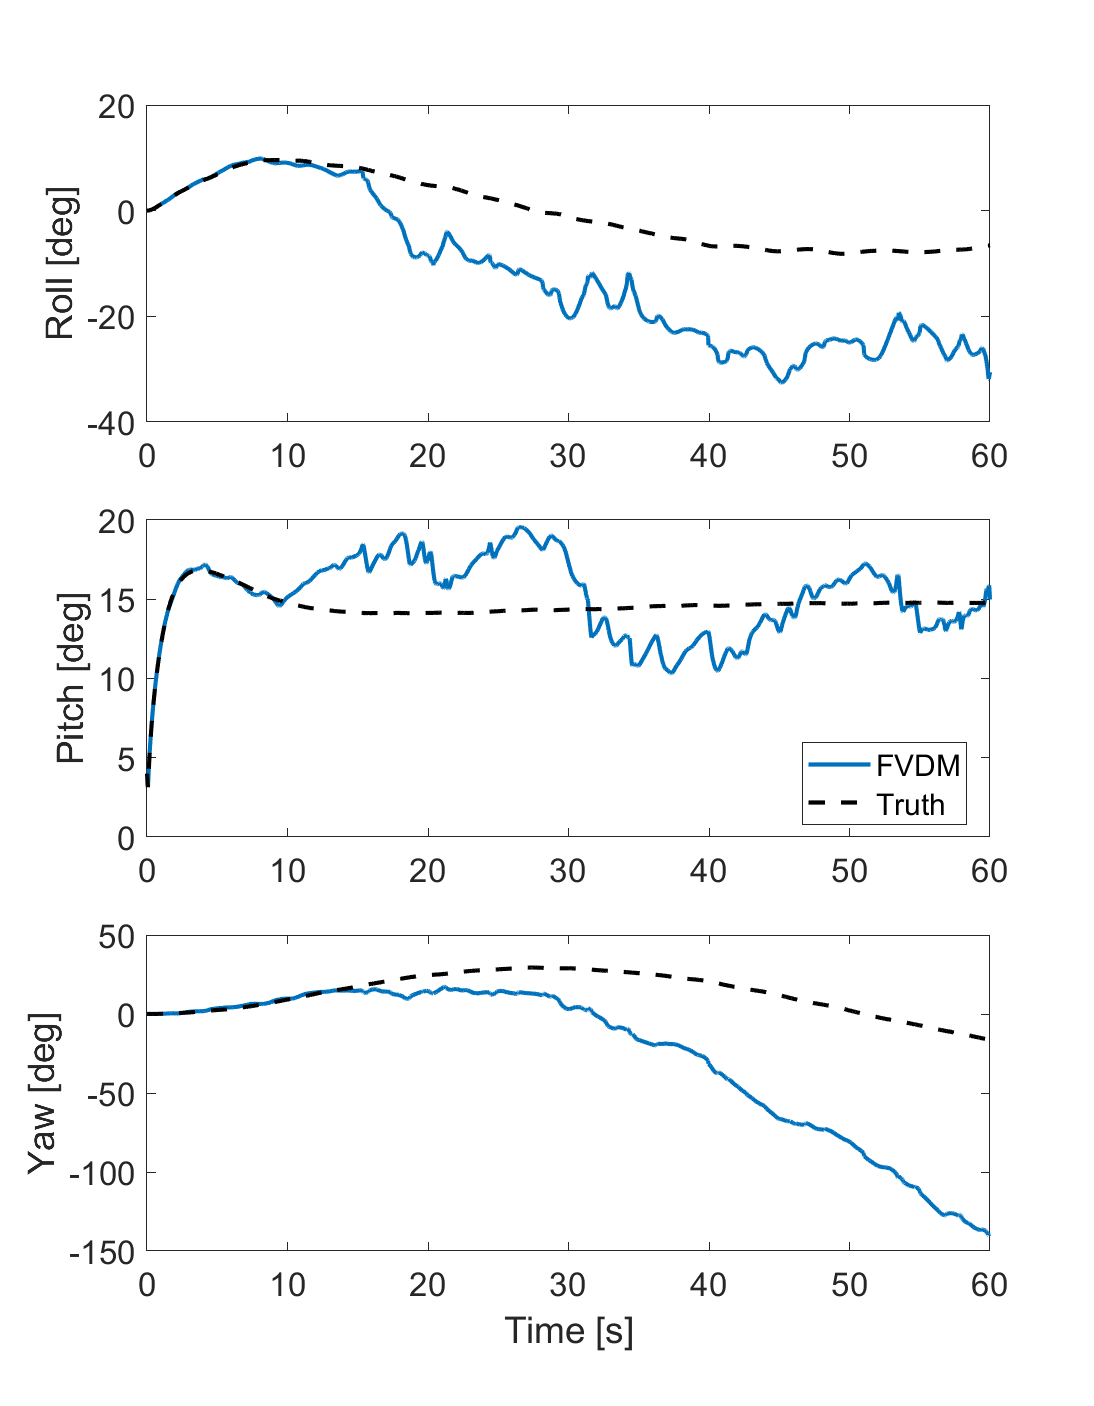
\includegraphics[width=1\linewidth]{Figures/dynamic/15/EULERANGLES.png}
    \end{subfigure}
    \begin{subfigure}{.45\textwidth}
        \centering
        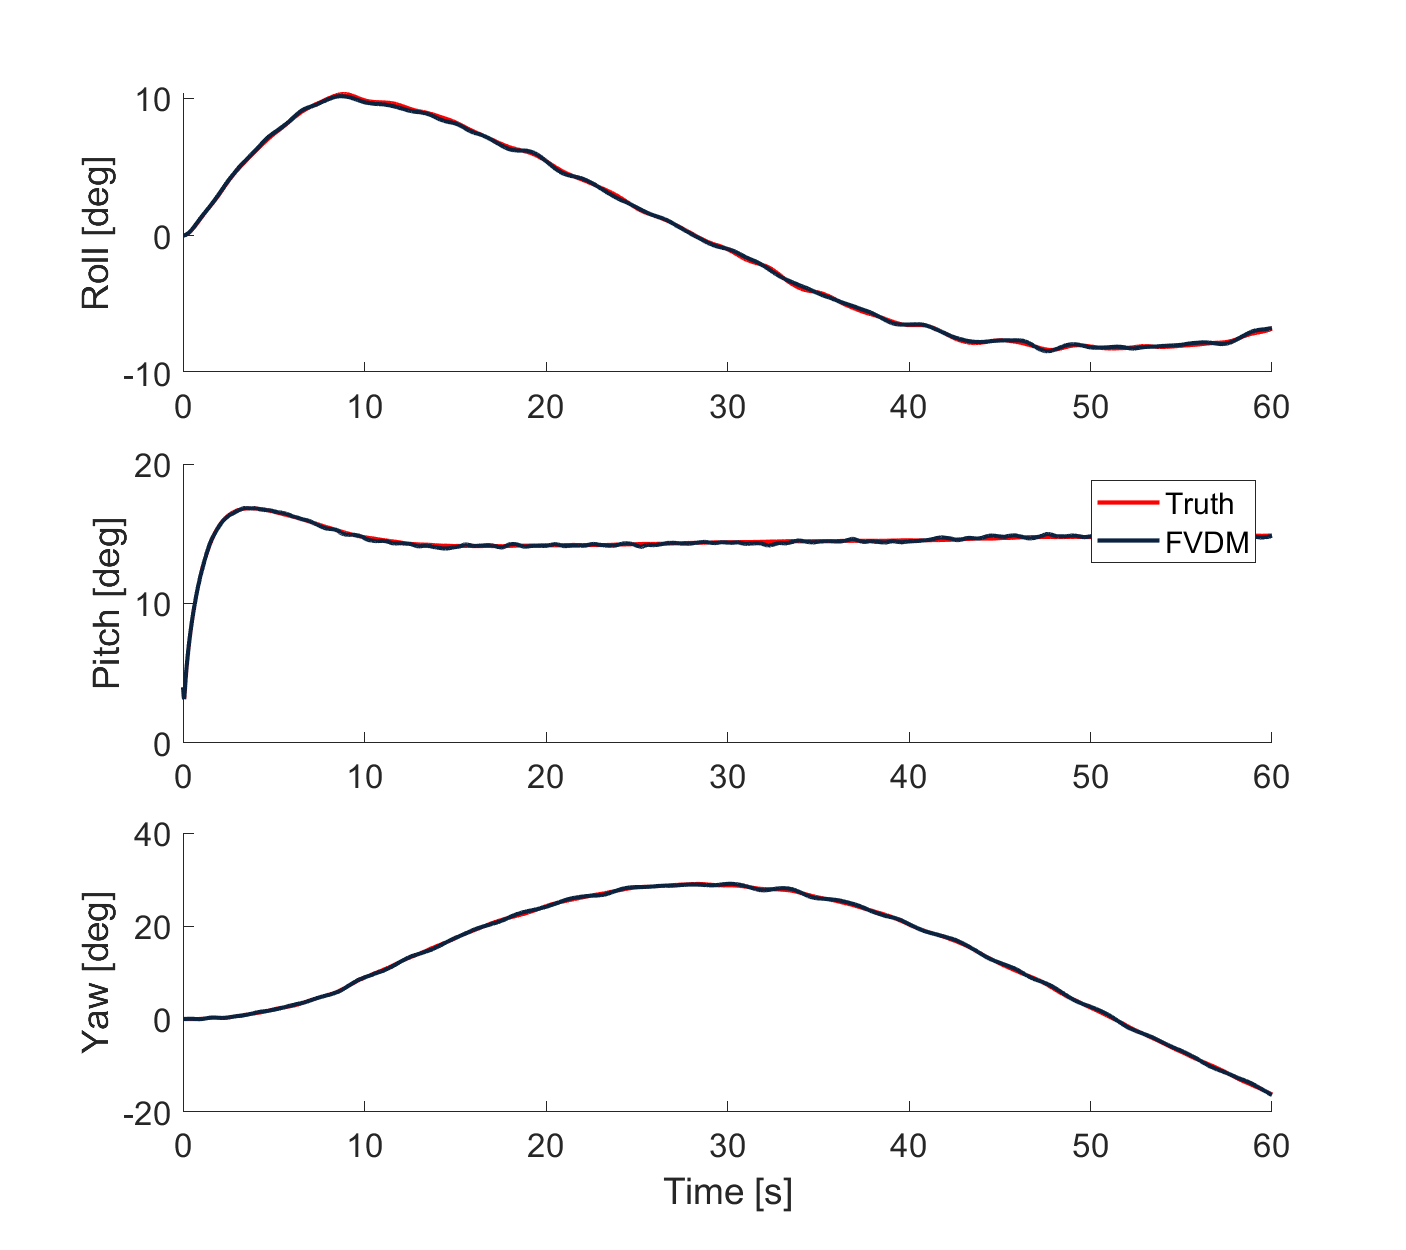
\includegraphics[width=1\linewidth]{Figures/dynamic/20/EULERANGLES.png}
    \end{subfigure}
    \caption{Average Euler attitude estimates of the FVDM and standard VDFLL implementation compared to the truth trajectory. The left figure is when both simulations had a signal power of \(15\) dB-Hz. The right figure is with a signal power of \(20\) dB-Hz.}\label{fig:EULER}
\end{figure}

Because the Euler attitude estimates are the integral of the angular rate estimate, barring the rotation of \(C_{\omega}\) (Equation~\ref{eq:eulerRates}), it is clear that worse estimates of angular rates lead to drifting error in the Euler attitude estimates of the aircraft. If not corrected, this can lead to drifting position and velocity estimation at lower \(C/N_0\) levels. To maintain better estimates of the angular rates and Euler attitude, an IMU or additional hardware sensor could be tied-in with the FVDM to provide direct measurements of those states. Another option, although sub-optimal, would be the addition of a second GPS antenna, in which GPS course measurements could be calculated and provided to the filter. It should further be noted that GPS course and the yaw of the aircraft are not the same as discussed in Chapter 2.

The clock bias and clock drift estimates from both filters are analyzed for trajectory two. Similar to trajectory one, the receiver in trajectory two is embedded with an OCXO\@. And as mentioned previously, the performance of the clock bias and drifts estimates correspond with the accuracy of the position and velocity estimates, respectively. Figure~\ref{fig:Clocks3} presents the clock bias estimates for both filters subject to the dynamics of trajectory two and signal power degradation. Figure~\ref{fig:Clocks4} dictates the clock drifts estimates under the same circumstances.


\begin{figure}[!ht]
    \begin{subfigure}{.45\textwidth}
        \centering
        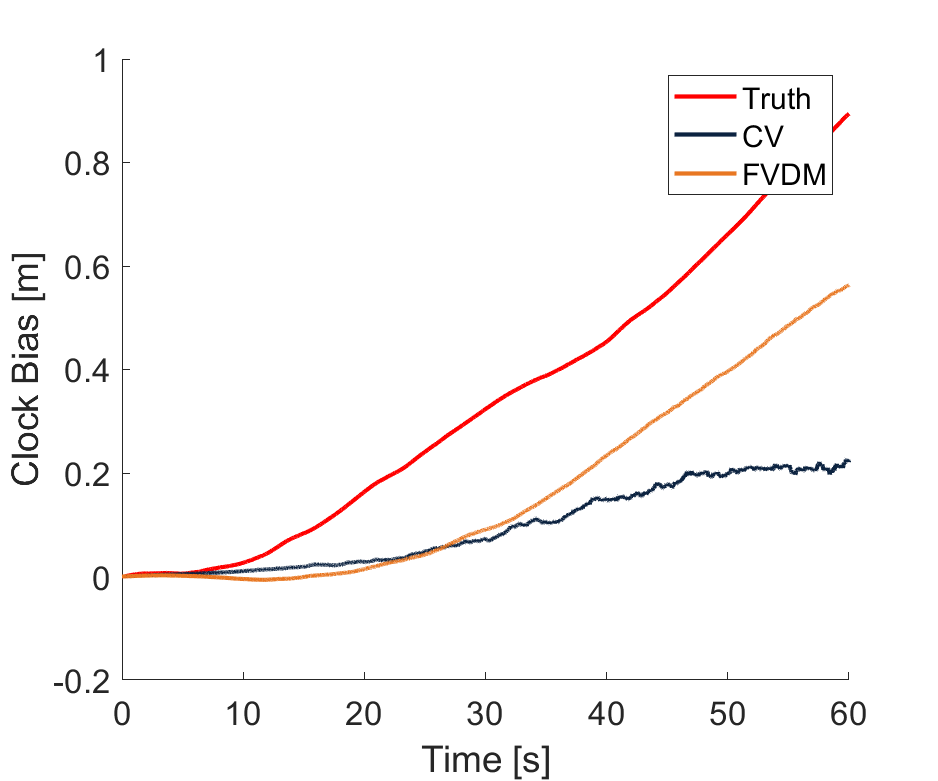
\includegraphics[width=1\linewidth]{Figures/dynamic/25/CLOCKBIAS.png}
    \end{subfigure}
    \begin{subfigure}{.45\textwidth}
        \centering
        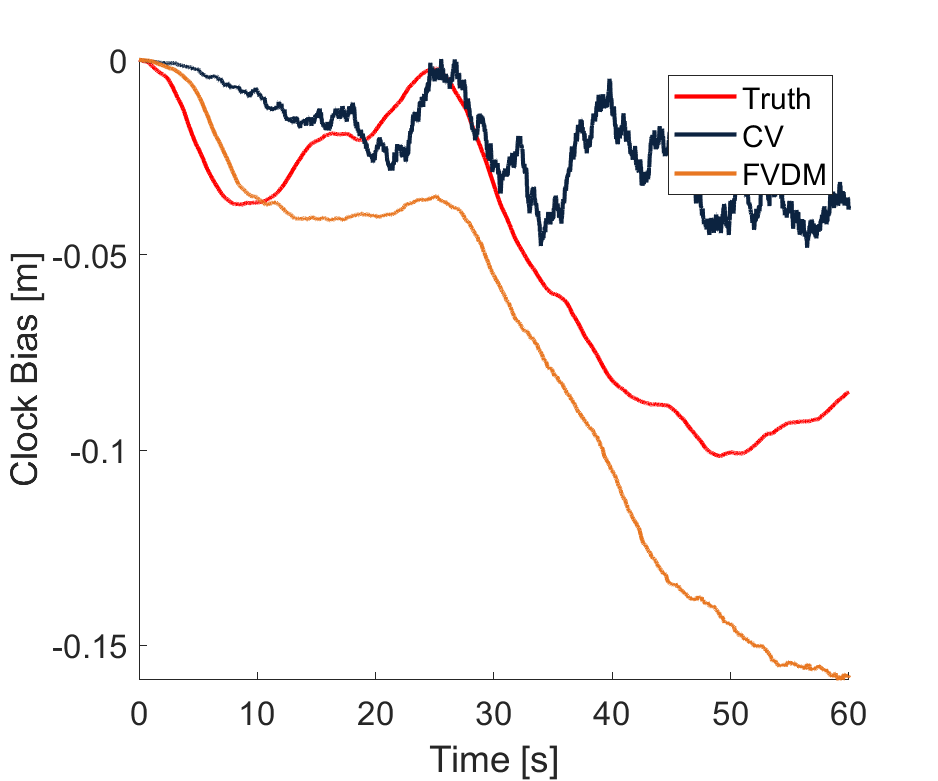
\includegraphics[width=1\linewidth]{Figures/dynamic/35/CLOCKBIAS.png}
    \end{subfigure}
    \caption{Average clock bias estimates of the FVDM and standard VDFLL implementation compared to the truth trajectory. The left figure is when both simulations had a signal power of \(20\) dB-Hz. The right figure is with a signal power of \(25\) dB-Hz.}\label{fig:Clocks3}
\end{figure}

\begin{figure}[!ht]
    \begin{subfigure}{.45\textwidth}
        \centering
        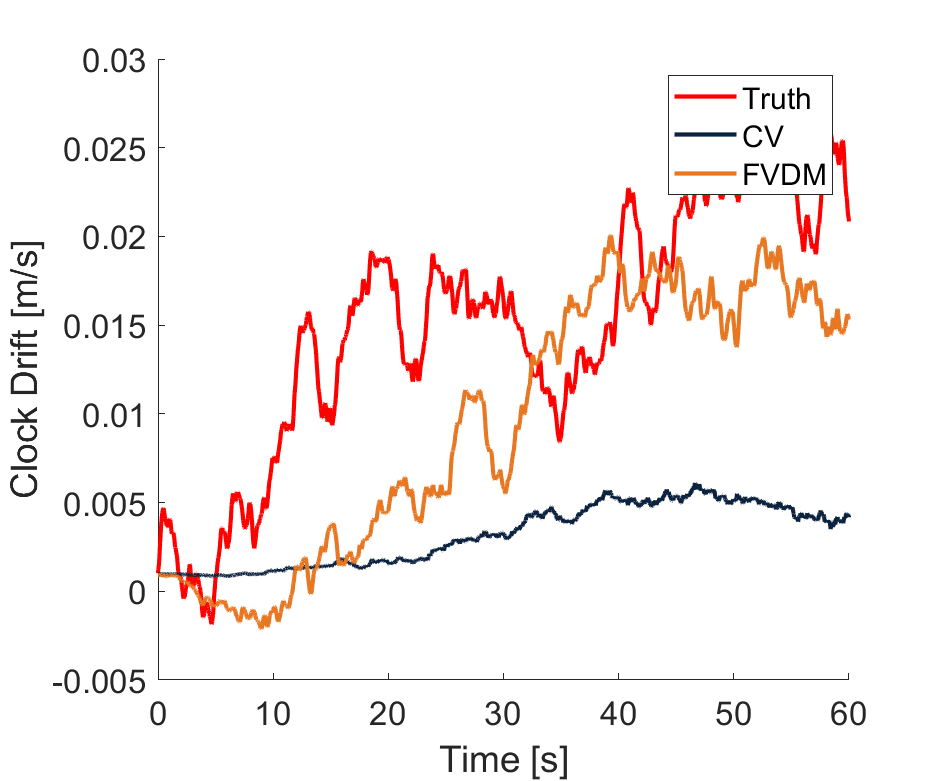
\includegraphics[width=1\linewidth]{Figures/dynamic/25/CLOCKDRIFT.png}
    \end{subfigure}
    \begin{subfigure}{.45\textwidth}
        \centering
        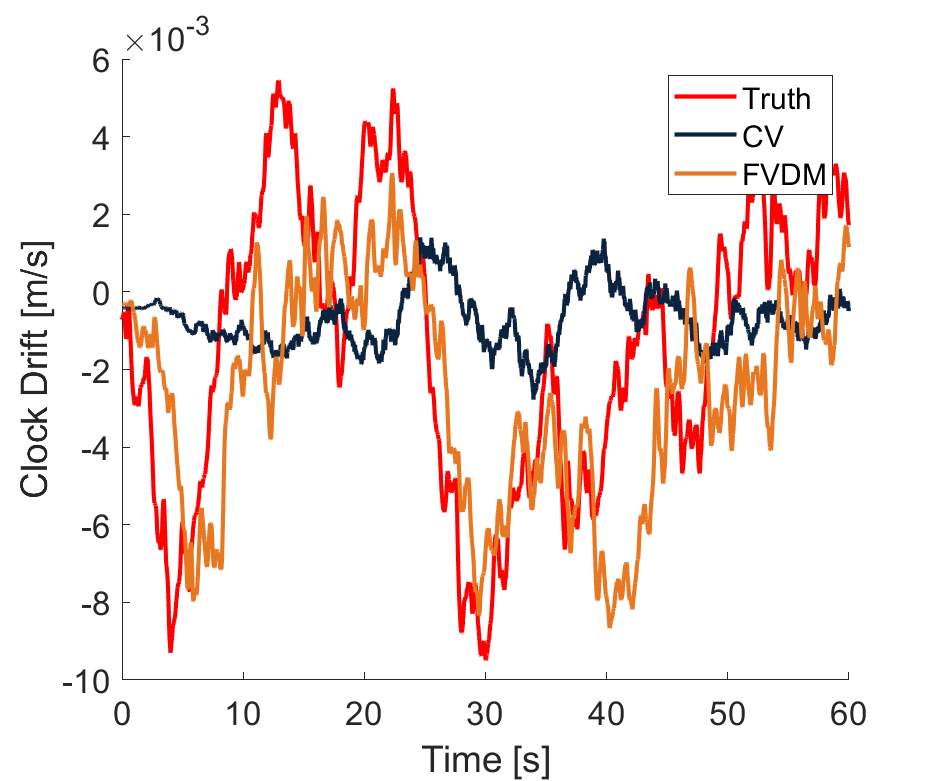
\includegraphics[width=1\linewidth]{Figures/dynamic/35/CLOCKDRIFT.png}
    \end{subfigure}
    \caption{Average clock drift estimates of the FVDM and standard VDFLL implementation compared to the truth trajectory. The left figure is when both simulations had a signal power of \(20\) dB-Hz. The right figure is with a signal power of \(25\) dB-Hz.}\label{fig:Clocks4}
\end{figure}

Lastly, Tables~\ref{tbl:dyn20FVDM} and~\ref{tbl:dyn20CV} provide the RMSE, STD, and maximum error calculated across the 100-run Monte Carlo simulation when the receiver is subject to interference that leaves the signal power at \(20\) dB-Hz.
\begin{table}[!ht]
    \caption{RMSE, STD, and maximum error from 100-run Monte Carlo simulation when the receiver is subject to a degraded signal power level of \(20\) dB-Hz.}\label{tbl:dyn20FVDM}
    \centering
    \begin{tabular}{ccccc}
        \toprule
                  & Position [m] & Speed [m/s] & Clock Bias [m] & Clock Drift [m/s] \\
        \midrule
        RMSE      & 0.64521      & 0.2673      & 0.1911         & 0.010044          \\
        STD       & 0.34121      & 0.12531     & 0.18278        & 0.0073514         \\
        Max Error & 1.5828       & 0.76501     & 0.5855         & 0.23049           \\
        \bottomrule
    \end{tabular}
\end{table}

\begin{table}[!ht]
    \caption{RMSE, STD, and maximum error from 100-run Monte Carlo simulation when the receiver is subject to a degraded signal power level of \(20\) dB-Hz.}\label{tbl:dyn20CV}
    \centering
    \begin{tabular}{ccccc}
        \toprule
                  & Position [m] & Speed [m/s] & Clock Bias [m] & Clock Drift [m/s] \\
        \midrule
        RMSE      & 196.98       & 6.0576      & 0.20098        & 0.010995          \\
        STD       & 126.68       & 0.92248     & 0.19358        & 0.0077631         \\
        Max Error & 431.72       & 8.468       & 0.62891        & 0.024964          \\
        \bottomrule
    \end{tabular}
\end{table}

% \begin{table}[!ht]
%     \caption{RMSE, STD, and maximum error from 100-run Monte Carlo simulation when the receiver is subject to a degraded signal power level of \(35\) dB-Hz.}\label{tbl:dyn35FVDM}
%     \centering
%     \begin{tabular}{ccccc}
%         \toprule
%                   & Position [m] & Speed [m/s] & Clock Bias [m] & Clock Drift [m/s] \\
%         \midrule
%         RMSE      & 0.023097     & 0.068845    & 0.028182       & 0.0026012         \\
%         STD       & 0.12219      & 0.03264     & 0.021298       & 0.0029319         \\
%         Max Error & 0.74388      & 0.28942     & 0.073095       & 0.008722          \\
%         \bottomrule
%     \end{tabular}
% \end{table}

% \begin{table}[!ht]
%     \caption{RMSE, STD, and maximum error from 100-run Monte Carlo simulation when the receiver is subject to a degraded signal power level of \(35\) dB-Hz.}\label{tbl:dyn35CV}
%     \centering
%     \begin{tabular}{ccccc}
%         \toprule
%                   & Position [m] & Speed [m/s] & Clock Bias [m] & Clock Drift [m/s] \\
%         \midrule
%         RMSE      & 0.097444     & 0.080918    & 0.030903       & 0.0033113         \\
%         STD       & 0.031969     & 0.035597    & 0.02659        & 0.0039156         \\
%         Max Error & 0.1905       & 0.23272     & 0.076362       & 0.00917           \\
%         \bottomrule
%     \end{tabular}
% \end{table}


\section{\textbf{Conclusions}}

This chapter presented a detailed explanation of the two trajectories used for the performance analysis of the proposed navigation filter compared to a standard, constant-velocity kinematic model VDFLL\@. Trajectory one is the baseline case where the aircraft is commanded to fly straight and maintain a constant altitude for the entirety of the simulation. Trajectory two is a more dynamic trajectory with alternating, banking turns throughout the simulation on top of the aircraft being commanded to climb and maintain an altitude of 1150 meters. Each trajectory was subject to a range of interferences starting from benign signal power to low signal power. Results from trajectory one show that when flying a standard, unexcited trajectory, the standard VDFLL and the proposed navigation filter are comparable. Results from trajectory two showcase the improved performance from the deeply-coupled FVDM because of the inability in the standard EKF to predict angular rates and Euler attitude. However, the results from trajectory two also show that the FVDM is not the sole-solution due to the unobservable angular states when excitement is lost in the simulated trajectory. External sensors such as a IMU or multi-antenna GPS system could improve the system observability for better estimates. Improvements to the proposed navigation filter are discussed in greater details in the next chapter.